\documentclass[12pt,a4paper]{article}

\usepackage[a4paper,text={16.5cm,25.2cm},centering]{geometry}
\usepackage{lmodern}
\usepackage{amssymb,amsmath}
\usepackage{bm}
\usepackage{graphicx}
\usepackage{microtype}
\usepackage{hyperref}
\setlength{\parindent}{0pt}
\setlength{\parskip}{1.2ex}

\hypersetup
       {   pdfauthor = { Kevin Corcoran },
           pdftitle={ Assignment \#1 },
           colorlinks=TRUE,
           linkcolor=black,
           citecolor=blue,
           urlcolor=blue
       }

\title{ Assignment \#1 }

\author{ Kevin Corcoran }


\usepackage{upquote}
\usepackage{listings}
\usepackage{xcolor}
\lstset{
    basicstyle=\ttfamily\footnotesize,
    upquote=true,
    breaklines=true,
    breakindent=0pt,
    keepspaces=true,
    showspaces=false,
    columns=fullflexible,
    showtabs=false,
    showstringspaces=false,
    escapeinside={(*@}{@*)},
    extendedchars=true,
}
\newcommand{\HLJLt}[1]{#1}
\newcommand{\HLJLw}[1]{#1}
\newcommand{\HLJLe}[1]{#1}
\newcommand{\HLJLeB}[1]{#1}
\newcommand{\HLJLo}[1]{#1}
\newcommand{\HLJLk}[1]{\textcolor[RGB]{148,91,176}{\textbf{#1}}}
\newcommand{\HLJLkc}[1]{\textcolor[RGB]{59,151,46}{\textit{#1}}}
\newcommand{\HLJLkd}[1]{\textcolor[RGB]{214,102,97}{\textit{#1}}}
\newcommand{\HLJLkn}[1]{\textcolor[RGB]{148,91,176}{\textbf{#1}}}
\newcommand{\HLJLkp}[1]{\textcolor[RGB]{148,91,176}{\textbf{#1}}}
\newcommand{\HLJLkr}[1]{\textcolor[RGB]{148,91,176}{\textbf{#1}}}
\newcommand{\HLJLkt}[1]{\textcolor[RGB]{148,91,176}{\textbf{#1}}}
\newcommand{\HLJLn}[1]{#1}
\newcommand{\HLJLna}[1]{#1}
\newcommand{\HLJLnb}[1]{#1}
\newcommand{\HLJLnbp}[1]{#1}
\newcommand{\HLJLnc}[1]{#1}
\newcommand{\HLJLncB}[1]{#1}
\newcommand{\HLJLnd}[1]{\textcolor[RGB]{214,102,97}{#1}}
\newcommand{\HLJLne}[1]{#1}
\newcommand{\HLJLneB}[1]{#1}
\newcommand{\HLJLnf}[1]{\textcolor[RGB]{66,102,213}{#1}}
\newcommand{\HLJLnfm}[1]{\textcolor[RGB]{66,102,213}{#1}}
\newcommand{\HLJLnp}[1]{#1}
\newcommand{\HLJLnl}[1]{#1}
\newcommand{\HLJLnn}[1]{#1}
\newcommand{\HLJLno}[1]{#1}
\newcommand{\HLJLnt}[1]{#1}
\newcommand{\HLJLnv}[1]{#1}
\newcommand{\HLJLnvc}[1]{#1}
\newcommand{\HLJLnvg}[1]{#1}
\newcommand{\HLJLnvi}[1]{#1}
\newcommand{\HLJLnvm}[1]{#1}
\newcommand{\HLJLl}[1]{#1}
\newcommand{\HLJLld}[1]{\textcolor[RGB]{148,91,176}{\textit{#1}}}
\newcommand{\HLJLs}[1]{\textcolor[RGB]{201,61,57}{#1}}
\newcommand{\HLJLsa}[1]{\textcolor[RGB]{201,61,57}{#1}}
\newcommand{\HLJLsb}[1]{\textcolor[RGB]{201,61,57}{#1}}
\newcommand{\HLJLsc}[1]{\textcolor[RGB]{201,61,57}{#1}}
\newcommand{\HLJLsd}[1]{\textcolor[RGB]{201,61,57}{#1}}
\newcommand{\HLJLsdB}[1]{\textcolor[RGB]{201,61,57}{#1}}
\newcommand{\HLJLsdC}[1]{\textcolor[RGB]{201,61,57}{#1}}
\newcommand{\HLJLse}[1]{\textcolor[RGB]{59,151,46}{#1}}
\newcommand{\HLJLsh}[1]{\textcolor[RGB]{201,61,57}{#1}}
\newcommand{\HLJLsi}[1]{#1}
\newcommand{\HLJLso}[1]{\textcolor[RGB]{201,61,57}{#1}}
\newcommand{\HLJLsr}[1]{\textcolor[RGB]{201,61,57}{#1}}
\newcommand{\HLJLss}[1]{\textcolor[RGB]{201,61,57}{#1}}
\newcommand{\HLJLssB}[1]{\textcolor[RGB]{201,61,57}{#1}}
\newcommand{\HLJLnB}[1]{\textcolor[RGB]{59,151,46}{#1}}
\newcommand{\HLJLnbB}[1]{\textcolor[RGB]{59,151,46}{#1}}
\newcommand{\HLJLnfB}[1]{\textcolor[RGB]{59,151,46}{#1}}
\newcommand{\HLJLnh}[1]{\textcolor[RGB]{59,151,46}{#1}}
\newcommand{\HLJLni}[1]{\textcolor[RGB]{59,151,46}{#1}}
\newcommand{\HLJLnil}[1]{\textcolor[RGB]{59,151,46}{#1}}
\newcommand{\HLJLnoB}[1]{\textcolor[RGB]{59,151,46}{#1}}
\newcommand{\HLJLoB}[1]{\textcolor[RGB]{102,102,102}{\textbf{#1}}}
\newcommand{\HLJLow}[1]{\textcolor[RGB]{102,102,102}{\textbf{#1}}}
\newcommand{\HLJLp}[1]{#1}
\newcommand{\HLJLc}[1]{\textcolor[RGB]{153,153,119}{\textit{#1}}}
\newcommand{\HLJLch}[1]{\textcolor[RGB]{153,153,119}{\textit{#1}}}
\newcommand{\HLJLcm}[1]{\textcolor[RGB]{153,153,119}{\textit{#1}}}
\newcommand{\HLJLcp}[1]{\textcolor[RGB]{153,153,119}{\textit{#1}}}
\newcommand{\HLJLcpB}[1]{\textcolor[RGB]{153,153,119}{\textit{#1}}}
\newcommand{\HLJLcs}[1]{\textcolor[RGB]{153,153,119}{\textit{#1}}}
\newcommand{\HLJLcsB}[1]{\textcolor[RGB]{153,153,119}{\textit{#1}}}
\newcommand{\HLJLg}[1]{#1}
\newcommand{\HLJLgd}[1]{#1}
\newcommand{\HLJLge}[1]{#1}
\newcommand{\HLJLgeB}[1]{#1}
\newcommand{\HLJLgh}[1]{#1}
\newcommand{\HLJLgi}[1]{#1}
\newcommand{\HLJLgo}[1]{#1}
\newcommand{\HLJLgp}[1]{#1}
\newcommand{\HLJLgs}[1]{#1}
\newcommand{\HLJLgsB}[1]{#1}
\newcommand{\HLJLgt}[1]{#1}


\begin{document}

\maketitle

\textbf{Including packages}

Most functions I've written in the DiffyQ.jl module. I did this in order to make the code, and this report a little cleaner. I have explicitely written the implicit methods in this report like backwards Euler and the Tapezoid method.


\begin{lstlisting}
(*@\HLJLk{using}@*) (*@\HLJLn{Plots}@*)
(*@\HLJLk{using}@*) (*@\HLJLn{LaTeXStrings}@*)
(*@\HLJLcs{{\#}}@*) (*@\HLJLcs{Load}@*) (*@\HLJLcs{DiffyQ}@*) (*@\HLJLcs{Module}@*) (*@\HLJLcs{and}@*) (*@\HLJLcs{required}@*) (*@\HLJLcs{functions}@*)
(*@\HLJLk{using}@*) (*@\HLJLn{Pkg}@*)
(*@\HLJLn{Pkg}@*)(*@\HLJLoB{.}@*)(*@\HLJLnf{activate}@*)(*@\HLJLp{(}@*)(*@\HLJLs{"{}DiffyQ"{}}@*)(*@\HLJLp{)}@*)
(*@\HLJLnf{include}@*)(*@\HLJLp{(}@*)(*@\HLJLs{"{}code/DiffyQ.jl"{}}@*)(*@\HLJLp{)}@*) (*@\HLJLcs{{\#}}@*) (*@\HLJLcs{Makes}@*) (*@\HLJLcs{sure}@*) (*@\HLJLcs{the}@*) (*@\HLJLcs{module}@*) (*@\HLJLcs{is}@*) (*@\HLJLcs{run}@*) (*@\HLJLcs{before}@*) (*@\HLJLcs{using}@*) (*@\HLJLcs{it}@*)
(*@\HLJLk{using}@*) (*@\HLJLoB{.}@*)(*@\HLJLn{DiffyQ}@*)(*@\HLJLoB{:}@*) (*@\HLJLn{CompTrapezoid}@*)(*@\HLJLp{,}@*) (*@\HLJLn{CompSimpson}@*)(*@\HLJLp{,}@*) (*@\HLJLn{Newtons}@*)(*@\HLJLp{,}@*) (*@\HLJLn{Euler}@*)(*@\HLJLp{,}@*) (*@\HLJLn{Midpoint2Step}@*)
\end{lstlisting}


\section{Problem 1}
 
Assuming  $Nh\leq T$ and
\[
E_{n+1} \leq (1+ch)E_n + h^2 
.\] 

Show
\[
  E_N \leq \frac{h}{c} \left(e^{ct}-1\right)
.\] 


Expanding the recursive definition
\begin{align*}
  E_{n+1} &\leq (1+ch)E_n + h^2 \leq (1+ch) \left((1+ch)E_{n-1} +h^2\right)
  + h^2 \\
          &\leq \dots \\
          &\leq h^2 \sum^{n}_{k=0} \left(1+ch\right)^k
\end{align*}

Setting n = N-1 and multiplying by $(1+ch)^{-N}$
\begin{align*}
  E_N &\leq h^2 \sum^{N-1}_{k=0} \left(1+ch\right)^k \\
  (1+ch)^{-N}E_N &\leq h^2 \sum^{N-1}_{k=0} \left(1+ch\right)^{-(k+1)}
\end{align*}

Using the geometric series and simplifying
\begin{align*}
  (1+ch)^{-N}E_N &\leq h^2 \sum^{N-1}_{k=0} \left(1+ch\right)^{-(k+1)} \\
                 &= h^2 (1+ch)^{-1} \frac{1-(1+ch)^{-N}}{1-(1+ch)^{-1}}\\
                 &= \frac{h}{c} \left(1-(1+ch)^{-N}\right)
\end{align*}

Multiplying by $(1+ch)^{N}$ and using $1+ch\leq e^{ch} \leq e^{c \frac{T}{N}}$

\begin{align*}
  E_N &\leq \frac{h}{c} \left((1+ch)^{N}-1\right) \\
      &\leq \frac{h}{c} (e^{cT} - 1)
\end{align*}

\section{Problem 2}
Solve 
\[
  \int_{{1}}^{{3}} {\sqrt{2+\cos^3(x)}e^{\sin(x)}} \: d{x} {}
.\] 
using the \emph{Composite Simpson} and \emph{Composite Trapezoid} Rule.  Then
estimate the error using formula $E(h) = \frac{|T(h)-T(h/2)|}{1-1/2^p}$.
Finally, plot the result on a $\log\log$ plot.


\textbf{Run simulations for $N = 2^2, 2^3, \ensuremath{\ldots},2^{10}$}


\begin{lstlisting}
(*@\HLJLcs{{\#}}@*) (*@\HLJLcs{function}@*) (*@\HLJLcs{to}@*) (*@\HLJLcs{be}@*) (*@\HLJLcs{integrated}@*) (*@\HLJLcs{from}@*) (*@\HLJLcs{a}@*) (*@\HLJLcs{to}@*) (*@\HLJLcs{b}@*)
(*@\HLJLnf{f}@*)(*@\HLJLp{(}@*)(*@\HLJLn{t}@*)(*@\HLJLp{)}@*) (*@\HLJLoB{=}@*) (*@\HLJLnf{sqrt}@*)(*@\HLJLp{(}@*)(*@\HLJLni{2}@*) (*@\HLJLoB{+}@*) (*@\HLJLnf{cos}@*)(*@\HLJLp{(}@*)(*@\HLJLn{t}@*)(*@\HLJLp{)}@*)(*@\HLJLoB{{\textasciicircum}}@*)(*@\HLJLni{3}@*)(*@\HLJLp{)}@*)(*@\HLJLoB{*}@*)(*@\HLJLnf{exp}@*)(*@\HLJLp{(}@*)(*@\HLJLnf{sin}@*)(*@\HLJLp{(}@*)(*@\HLJLn{t}@*)(*@\HLJLp{))}@*)

(*@\HLJLn{a}@*) (*@\HLJLoB{=}@*) (*@\HLJLni{1}@*)(*@\HLJLp{;}@*) (*@\HLJLn{b}@*) (*@\HLJLoB{=}@*) (*@\HLJLni{3}@*)(*@\HLJLp{;}@*) (*@\HLJLcm{{\#}=}@*) (*@\HLJLcm{N}@*) (*@\HLJLcm{=}@*) (*@\HLJLcm{2{\textasciicircum}(10);}@*) (*@\HLJLcm{={\#}}@*) (*@\HLJLn{T}@*) (*@\HLJLoB{=}@*) (*@\HLJLn{b}@*)(*@\HLJLoB{-}@*)(*@\HLJLn{a}@*)(*@\HLJLp{;}@*)

(*@\HLJLcs{{\#}}@*) (*@\HLJLcs{Plotting}@*) (*@\HLJLcs{error}@*) (*@\HLJLcs{routine}@*)
(*@\HLJLn{NList}@*) (*@\HLJLoB{=}@*) (*@\HLJLni{2}@*) (*@\HLJLoB{.{\textasciicircum}}@*)(*@\HLJLp{(}@*)(*@\HLJLni{2}@*)(*@\HLJLoB{:}@*)(*@\HLJLni{10}@*)(*@\HLJLp{)}@*)
(*@\HLJLn{errTrapeList}@*) (*@\HLJLoB{=}@*) (*@\HLJLnf{zeros}@*)(*@\HLJLp{(}@*)(*@\HLJLnf{size}@*)(*@\HLJLp{(}@*)(*@\HLJLn{NList}@*)(*@\HLJLp{))}@*)
(*@\HLJLn{errSimpList}@*) (*@\HLJLoB{=}@*) (*@\HLJLnf{zeros}@*)(*@\HLJLp{(}@*)(*@\HLJLnf{size}@*)(*@\HLJLp{(}@*)(*@\HLJLn{NList}@*)(*@\HLJLp{))}@*)
(*@\HLJLk{for}@*) (*@\HLJLn{i}@*) (*@\HLJLoB{=}@*) (*@\HLJLni{1}@*) (*@\HLJLoB{:}@*) (*@\HLJLnf{length}@*)(*@\HLJLp{(}@*)(*@\HLJLn{NList}@*)(*@\HLJLp{)}@*)
    (*@\HLJLn{N}@*) (*@\HLJLoB{=}@*) (*@\HLJLn{NList}@*)(*@\HLJLp{[}@*)(*@\HLJLn{i}@*)(*@\HLJLp{]}@*)

    (*@\HLJLn{utrape}@*) (*@\HLJLoB{=}@*) (*@\HLJLnf{CompTrapezoid}@*)(*@\HLJLp{(}@*)(*@\HLJLn{N}@*)(*@\HLJLp{,}@*)(*@\HLJLn{a}@*)(*@\HLJLp{,}@*)(*@\HLJLn{b}@*)(*@\HLJLp{,}@*)(*@\HLJLn{f}@*)(*@\HLJLp{)}@*)
    (*@\HLJLn{utexact}@*) (*@\HLJLoB{=}@*) (*@\HLJLnf{CompTrapezoid}@*)(*@\HLJLp{(}@*)(*@\HLJLni{2}@*)(*@\HLJLoB{*}@*)(*@\HLJLn{N}@*)(*@\HLJLp{,}@*)(*@\HLJLn{a}@*)(*@\HLJLp{,}@*)(*@\HLJLn{b}@*)(*@\HLJLp{,}@*)(*@\HLJLn{f}@*)(*@\HLJLp{)}@*)

    (*@\HLJLn{usimps}@*) (*@\HLJLoB{=}@*) (*@\HLJLnf{CompSimpson}@*)(*@\HLJLp{(}@*)(*@\HLJLn{N}@*)(*@\HLJLp{,}@*)(*@\HLJLn{a}@*)(*@\HLJLp{,}@*)(*@\HLJLn{b}@*)(*@\HLJLp{,}@*)(*@\HLJLn{f}@*)(*@\HLJLp{)}@*)
    (*@\HLJLn{usexact}@*) (*@\HLJLoB{=}@*) (*@\HLJLnf{CompSimpson}@*)(*@\HLJLp{(}@*)(*@\HLJLni{2}@*)(*@\HLJLoB{*}@*)(*@\HLJLn{N}@*)(*@\HLJLp{,}@*)(*@\HLJLn{a}@*)(*@\HLJLp{,}@*)(*@\HLJLn{b}@*)(*@\HLJLp{,}@*)(*@\HLJLn{f}@*)(*@\HLJLp{)}@*)

    (*@\HLJLcs{{\#}}@*) (*@\HLJLcs{estimate}@*) (*@\HLJLcs{error}@*)
    (*@\HLJLn{errTrapeList}@*)(*@\HLJLp{[}@*)(*@\HLJLn{i}@*)(*@\HLJLp{]}@*) (*@\HLJLoB{=}@*) (*@\HLJLnf{abs}@*)(*@\HLJLp{(}@*)(*@\HLJLn{utrape}@*)(*@\HLJLoB{-}@*)(*@\HLJLn{utexact}@*)(*@\HLJLp{)}@*)(*@\HLJLoB{./}@*)(*@\HLJLp{(}@*)(*@\HLJLni{1}@*)(*@\HLJLoB{-}@*)(*@\HLJLp{(}@*)(*@\HLJLni{1}@*)(*@\HLJLoB{/}@*)(*@\HLJLni{2}@*)(*@\HLJLoB{{\textasciicircum}}@*)(*@\HLJLni{2}@*)(*@\HLJLp{))}@*)
    (*@\HLJLn{errSimpList}@*)(*@\HLJLp{[}@*)(*@\HLJLn{i}@*)(*@\HLJLp{]}@*) (*@\HLJLoB{=}@*) (*@\HLJLnf{abs}@*)(*@\HLJLp{(}@*)(*@\HLJLn{usimps}@*)(*@\HLJLoB{-}@*)(*@\HLJLn{usexact}@*)(*@\HLJLp{)}@*)(*@\HLJLoB{./}@*)(*@\HLJLp{(}@*)(*@\HLJLni{1}@*)(*@\HLJLoB{-}@*)(*@\HLJLp{(}@*)(*@\HLJLni{1}@*)(*@\HLJLoB{/}@*)(*@\HLJLni{2}@*)(*@\HLJLoB{{\textasciicircum}}@*)(*@\HLJLni{4}@*)(*@\HLJLp{))}@*)
(*@\HLJLk{end}@*)

(*@\HLJLnf{plot}@*)(*@\HLJLp{(}@*)(*@\HLJLn{T}@*)(*@\HLJLoB{./}@*)(*@\HLJLn{NList}@*)(*@\HLJLp{,}@*) (*@\HLJLn{errTrapeList}@*)(*@\HLJLp{,}@*)(*@\HLJLn{label}@*)(*@\HLJLoB{=}@*)(*@\HLJLs{"{}Trapezoid"{}}@*)(*@\HLJLp{,}@*)(*@\HLJLn{xaxis}@*)(*@\HLJLoB{=:}@*)(*@\HLJLn{log}@*)(*@\HLJLp{,}@*)(*@\HLJLn{yaxis}@*)(*@\HLJLoB{=:}@*)(*@\HLJLn{log}@*)(*@\HLJLp{,}@*) (*@\HLJLn{marker}@*) (*@\HLJLoB{=}@*) (*@\HLJLp{(}@*)(*@\HLJLsc{:dot}@*)(*@\HLJLp{,}@*)(*@\HLJLni{5}@*)(*@\HLJLp{),}@*) (*@\HLJLn{add{\_}marker}@*) (*@\HLJLoB{=}@*) (*@\HLJLkc{true}@*)(*@\HLJLp{)}@*)
(*@\HLJLnf{plot!}@*)(*@\HLJLp{(}@*)(*@\HLJLn{T}@*)(*@\HLJLoB{./}@*)(*@\HLJLn{NList}@*)(*@\HLJLp{,}@*) (*@\HLJLn{errSimpList}@*)(*@\HLJLp{,}@*)(*@\HLJLn{label}@*)(*@\HLJLoB{=}@*)(*@\HLJLs{"{}Simpson"{}}@*)(*@\HLJLp{,}@*)(*@\HLJLn{xaxis}@*)(*@\HLJLoB{=:}@*)(*@\HLJLn{log}@*)(*@\HLJLp{,}@*)(*@\HLJLn{yaxis}@*)(*@\HLJLoB{=:}@*)(*@\HLJLn{log}@*)(*@\HLJLp{,}@*) (*@\HLJLn{marker}@*) (*@\HLJLoB{=}@*) (*@\HLJLp{(}@*)(*@\HLJLsc{:square}@*)(*@\HLJLp{,}@*)(*@\HLJLni{5}@*)(*@\HLJLp{),}@*) (*@\HLJLn{add{\_}marker}@*) (*@\HLJLoB{=}@*) (*@\HLJLkc{true}@*)(*@\HLJLp{)}@*)
(*@\HLJLnf{xlabel!}@*)(*@\HLJLp{(}@*)(*@\HLJLs{"{}Stepsize"{}}@*)(*@\HLJLp{)}@*)
(*@\HLJLnf{ylabel!}@*)(*@\HLJLp{(}@*)(*@\HLJLs{"{}Approximate}@*) (*@\HLJLs{Error"{}}@*)(*@\HLJLp{)}@*)
\end{lstlisting}

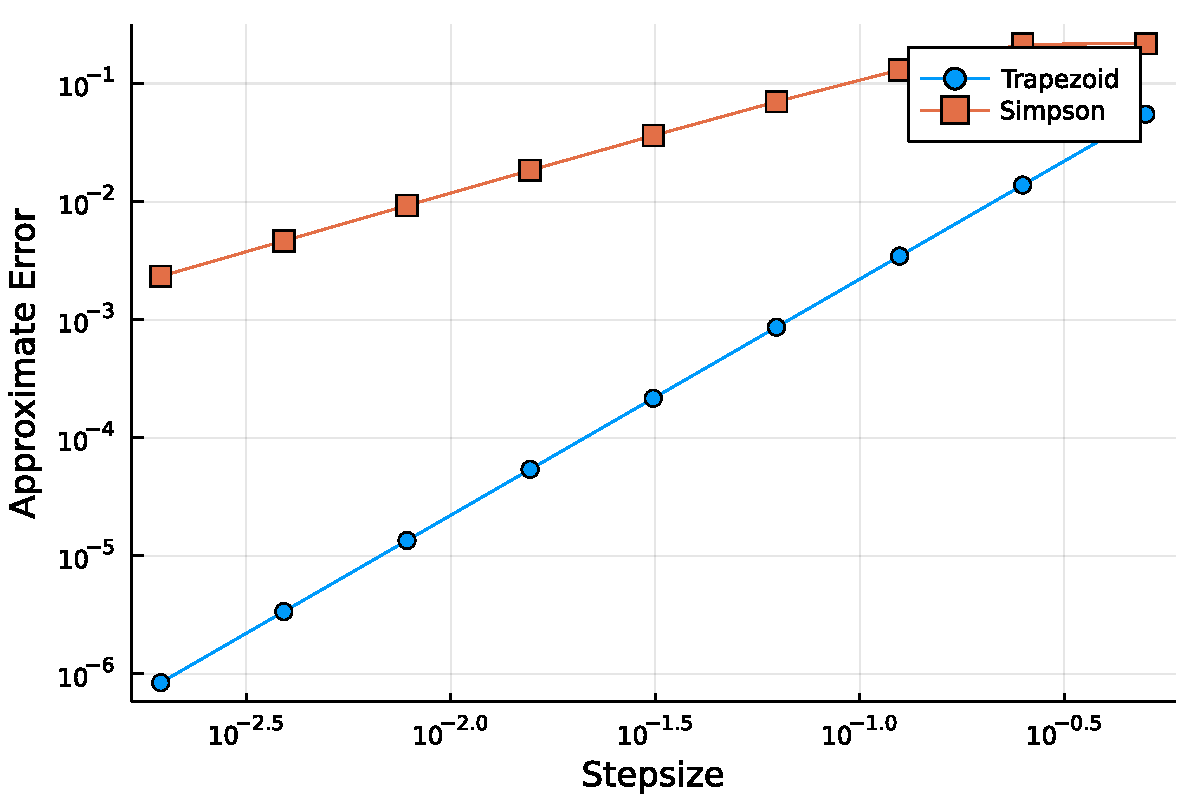
\includegraphics[width=\linewidth]{figures/ass_1_report_2_1.pdf}

\section{Problem 3}
Implement Newton's method to solve the non-linear equation for 0

$x-\alpha+\beta\sinh\left( x - \cos(s-1) \right) = 0$

\textbf{Defining variables}


\begin{lstlisting}
(*@\HLJLn{\ensuremath{\alpha}}@*) (*@\HLJLoB{=}@*) (*@\HLJLnfB{0.9}@*)
(*@\HLJLn{\ensuremath{\beta}}@*) (*@\HLJLoB{=}@*) (*@\HLJLnfB{50000.0}@*)
(*@\HLJLcs{{\#}}@*) (*@\HLJLcs{equation}@*) (*@\HLJLcs{to}@*) (*@\HLJLcs{solve}@*)
(*@\HLJLnf{f}@*)(*@\HLJLp{(}@*)(*@\HLJLn{x}@*)(*@\HLJLp{,}@*)(*@\HLJLn{s}@*)(*@\HLJLp{)}@*) (*@\HLJLoB{=}@*) (*@\HLJLn{x}@*) (*@\HLJLoB{-}@*) (*@\HLJLn{\ensuremath{\alpha}}@*) (*@\HLJLoB{+}@*) (*@\HLJLn{\ensuremath{\beta}}@*)(*@\HLJLoB{*}@*)(*@\HLJLnf{sinh}@*)(*@\HLJLp{(}@*)(*@\HLJLn{x}@*)(*@\HLJLoB{-}@*)(*@\HLJLnf{cos}@*)(*@\HLJLp{(}@*)(*@\HLJLn{s}@*)(*@\HLJLoB{-}@*)(*@\HLJLni{1}@*)(*@\HLJLp{))}@*)
(*@\HLJLcs{{\#}}@*) (*@\HLJLcs{derivative}@*) (*@\HLJLcs{of}@*) (*@\HLJLcs{equation}@*)
(*@\HLJLnf{df}@*)(*@\HLJLp{(}@*)(*@\HLJLn{x}@*)(*@\HLJLp{,}@*)(*@\HLJLn{s}@*)(*@\HLJLp{)}@*) (*@\HLJLoB{=}@*) (*@\HLJLni{1}@*) (*@\HLJLoB{+}@*) (*@\HLJLn{\ensuremath{\beta}}@*)(*@\HLJLoB{*}@*)(*@\HLJLnf{cosh}@*)(*@\HLJLp{(}@*)(*@\HLJLn{x}@*)(*@\HLJLoB{-}@*)(*@\HLJLnf{cos}@*)(*@\HLJLp{(}@*)(*@\HLJLn{s}@*)(*@\HLJLoB{-}@*)(*@\HLJLni{1}@*)(*@\HLJLp{))}@*)
(*@\HLJLcs{{\#}}@*) (*@\HLJLcs{initial}@*) (*@\HLJLcs{guess}@*)
(*@\HLJLn{x0}@*) (*@\HLJLoB{=}@*) (*@\HLJLnfB{2.0}@*)
\end{lstlisting}

\begin{lstlisting}
2.0
\end{lstlisting}


\textbf{Solving equation for various values of $s$}


\begin{lstlisting}
(*@\HLJLn{ss}@*) (*@\HLJLoB{=}@*) (*@\HLJLnfB{0.0}@*)(*@\HLJLoB{:}@*)(*@\HLJLnfB{0.1}@*)(*@\HLJLoB{:}@*)(*@\HLJLnfB{20.0}@*)

(*@\HLJLn{xs}@*) (*@\HLJLoB{=}@*) (*@\HLJLp{[]}@*)
(*@\HLJLk{for}@*) (*@\HLJLn{s}@*) (*@\HLJLkp{in}@*) (*@\HLJLn{ss}@*)
    (*@\HLJLnf{push!}@*)(*@\HLJLp{(}@*)(*@\HLJLn{xs}@*)(*@\HLJLp{,}@*)(*@\HLJLnf{Newtons}@*)(*@\HLJLp{(}@*)(*@\HLJLn{f}@*)(*@\HLJLp{,}@*)(*@\HLJLn{df}@*)(*@\HLJLp{,}@*)(*@\HLJLn{x0}@*)(*@\HLJLp{,}@*)(*@\HLJLn{s}@*)(*@\HLJLp{))}@*)
(*@\HLJLk{end}@*)
\end{lstlisting}


\textbf{Plotting x vs s and cos(s-1) on the same plot}


\begin{lstlisting}
(*@\HLJLnf{plot}@*)(*@\HLJLp{(}@*)(*@\HLJLn{ss}@*)(*@\HLJLp{,}@*)(*@\HLJLn{xs}@*)(*@\HLJLp{,}@*) (*@\HLJLn{label}@*) (*@\HLJLoB{=}@*) (*@\HLJLso{L"{}Newtons"{}}@*)(*@\HLJLp{,}@*)(*@\HLJLn{marker}@*) (*@\HLJLoB{=}@*) (*@\HLJLp{(}@*)(*@\HLJLsc{:dot}@*)(*@\HLJLp{,}@*)(*@\HLJLni{2}@*)(*@\HLJLp{),}@*) (*@\HLJLn{add{\_}marker}@*)(*@\HLJLoB{=}@*)(*@\HLJLkc{true}@*)(*@\HLJLp{,}@*) (*@\HLJLn{thickness{\_}scaling}@*) (*@\HLJLoB{=}@*) (*@\HLJLnfB{1.5}@*)(*@\HLJLp{)}@*)
(*@\HLJLnf{plot!}@*)(*@\HLJLp{(}@*)(*@\HLJLn{ss}@*)(*@\HLJLp{,}@*) (*@\HLJLn{cos}@*)(*@\HLJLoB{.}@*)(*@\HLJLp{(}@*)(*@\HLJLn{ss}@*)(*@\HLJLoB{.-}@*)(*@\HLJLni{1}@*)(*@\HLJLp{),}@*) (*@\HLJLn{label}@*) (*@\HLJLoB{=}@*) (*@\HLJLso{L"{}{\textbackslash}cos(s-1)"{}}@*)(*@\HLJLp{)}@*)
(*@\HLJLnf{xlabel!}@*)(*@\HLJLp{(}@*)(*@\HLJLs{"{}s"{}}@*)(*@\HLJLp{)}@*)
(*@\HLJLnf{ylabel!}@*)(*@\HLJLp{(}@*)(*@\HLJLs{"{}x"{}}@*)(*@\HLJLp{)}@*)
\end{lstlisting}

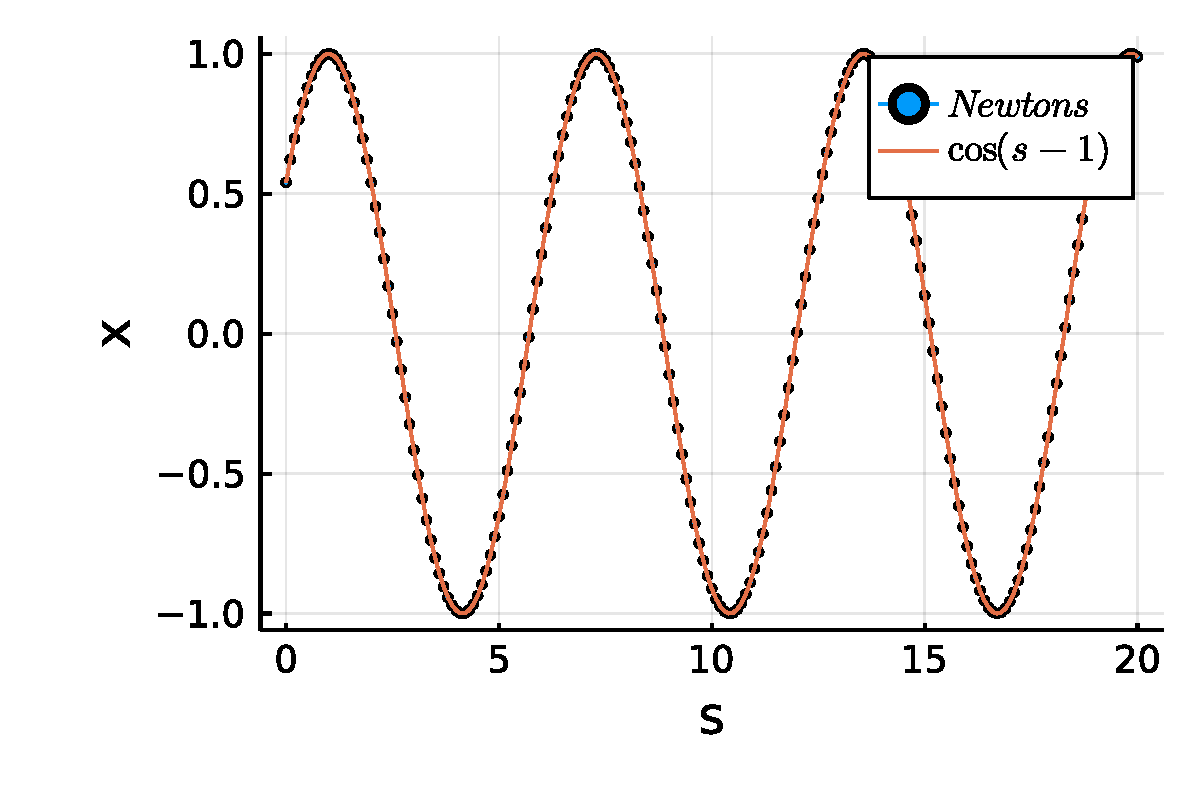
\includegraphics[width=\linewidth]{figures/ass_1_report_5_1.pdf}

\section{Problem 4}
\subsection{Part 1}
Solve the initial value problem using Eulers method for $T = 2^{-10}$ and various values of h.

\textbf{The solution when the stepsize is not small enough. We see that the solution is not bounded.}


\begin{lstlisting}
(*@\HLJLcs{{\#}}@*) (*@\HLJLcs{Differential}@*) (*@\HLJLcs{equation}@*)
(*@\HLJLnf{func}@*)(*@\HLJLp{(}@*)(*@\HLJLn{u}@*)(*@\HLJLp{,}@*) (*@\HLJLn{t}@*)(*@\HLJLp{,}@*) (*@\HLJLn{\ensuremath{\lambda}}@*)(*@\HLJLp{)}@*) (*@\HLJLoB{=}@*) (*@\HLJLoB{-}@*)(*@\HLJLn{\ensuremath{\lambda}}@*)(*@\HLJLoB{*}@*)(*@\HLJLnf{sinh}@*)(*@\HLJLp{(}@*)(*@\HLJLn{u}@*)(*@\HLJLoB{-}@*)(*@\HLJLnf{cos}@*)(*@\HLJLp{(}@*)(*@\HLJLn{t}@*)(*@\HLJLoB{-}@*)(*@\HLJLni{1}@*)(*@\HLJLp{))}@*)

(*@\HLJLcs{{\#}}@*) (*@\HLJLcs{defining}@*) (*@\HLJLcs{variables/initial}@*) (*@\HLJLcs{conditions}@*)
(*@\HLJLn{T}@*) (*@\HLJLoB{=}@*) (*@\HLJLnfB{2.0}@*)(*@\HLJLoB{{\textasciicircum}}@*)(*@\HLJLp{(}@*)(*@\HLJLoB{-}@*)(*@\HLJLnfB{10.0}@*)(*@\HLJLp{);}@*) (*@\HLJLn{t0}@*) (*@\HLJLoB{=}@*) (*@\HLJLni{0}@*)(*@\HLJLp{;}@*) (*@\HLJLn{u0}@*) (*@\HLJLoB{=}@*) (*@\HLJLni{0}@*)(*@\HLJLp{;}@*) (*@\HLJLn{\ensuremath{\lambda}}@*) (*@\HLJLoB{=}@*) (*@\HLJLnfB{10.0}@*)(*@\HLJLoB{{\textasciicircum}}@*)(*@\HLJLp{(}@*)(*@\HLJLnfB{6.0}@*)(*@\HLJLp{);}@*)

(*@\HLJLcs{{\#}}@*) (*@\HLJLcs{Foward}@*) (*@\HLJLcs{Euler}@*)
(*@\HLJLn{h0}@*) (*@\HLJLoB{=}@*) (*@\HLJLnfB{2.0}@*)(*@\HLJLoB{{\textasciicircum}}@*)(*@\HLJLp{(}@*)(*@\HLJLoB{-}@*)(*@\HLJLni{18}@*)(*@\HLJLp{);}@*)
(*@\HLJLn{N}@*) (*@\HLJLoB{=}@*) (*@\HLJLnf{Int}@*)(*@\HLJLp{(}@*)(*@\HLJLn{T}@*)(*@\HLJLoB{/}@*)(*@\HLJLp{(}@*)(*@\HLJLn{h0}@*)(*@\HLJLp{))}@*)
(*@\HLJLn{h}@*) (*@\HLJLoB{=}@*) (*@\HLJLn{T}@*)(*@\HLJLoB{/}@*)(*@\HLJLn{N}@*)

(*@\HLJLn{u}@*) (*@\HLJLoB{=}@*) (*@\HLJLnf{Euler}@*)(*@\HLJLp{(}@*)(*@\HLJLn{func}@*)(*@\HLJLp{,}@*)(*@\HLJLn{N}@*)(*@\HLJLp{,}@*)(*@\HLJLn{T}@*)(*@\HLJLp{,}@*)(*@\HLJLn{t0}@*)(*@\HLJLp{,}@*)(*@\HLJLn{u0}@*)(*@\HLJLp{,}@*)(*@\HLJLn{\ensuremath{\lambda}}@*)(*@\HLJLp{)}@*)
(*@\HLJLn{tList}@*) (*@\HLJLoB{=}@*) (*@\HLJLnf{collect}@*)(*@\HLJLp{(}@*)(*@\HLJLni{0}@*)(*@\HLJLoB{:}@*)(*@\HLJLn{N}@*)(*@\HLJLp{)}@*)(*@\HLJLoB{*}@*)(*@\HLJLp{(}@*)(*@\HLJLn{T}@*)(*@\HLJLoB{/}@*)(*@\HLJLn{N}@*)(*@\HLJLp{)}@*)
(*@\HLJLnf{plot}@*)(*@\HLJLp{(}@*)(*@\HLJLn{tList}@*)(*@\HLJLp{,}@*) (*@\HLJLn{u}@*)(*@\HLJLp{,}@*) (*@\HLJLn{label}@*) (*@\HLJLoB{=}@*) (*@\HLJLs{"{}Euler"{}}@*)(*@\HLJLp{)}@*)
(*@\HLJLnf{xlabel!}@*)(*@\HLJLp{(}@*)(*@\HLJLso{L"{}t"{}}@*)(*@\HLJLp{,}@*) (*@\HLJLn{thickness{\_}scaling}@*) (*@\HLJLoB{=}@*) (*@\HLJLnfB{1.5}@*)(*@\HLJLp{)}@*)
(*@\HLJLnf{ylabel!}@*)(*@\HLJLp{(}@*)(*@\HLJLso{L"{}u(t)"{}}@*)(*@\HLJLp{)}@*)
\end{lstlisting}

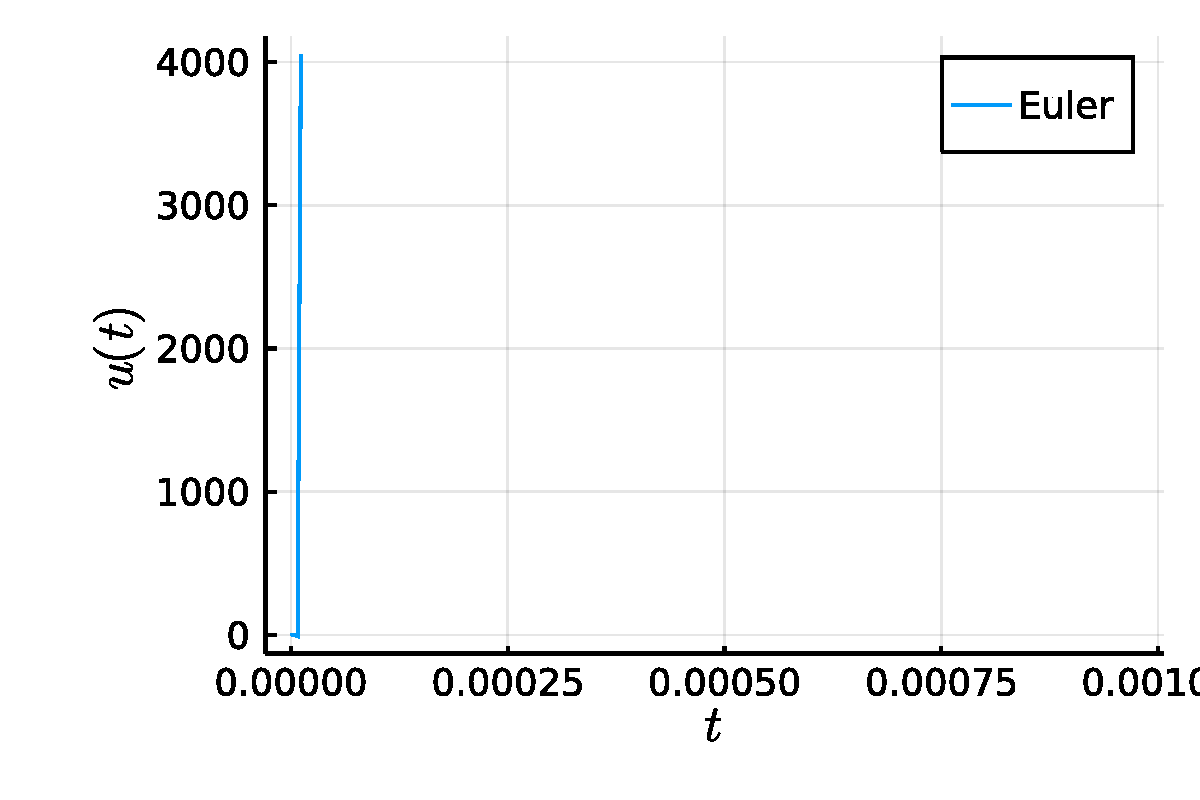
\includegraphics[width=\linewidth]{figures/ass_1_report_6_1.pdf}

\textbf{Stepsize at $h = 2^{-20}$ the solution becomes bounded}


\begin{lstlisting}
(*@\HLJLcs{{\#}}@*) (*@\HLJLcs{Foward}@*) (*@\HLJLcs{Euler}@*)
(*@\HLJLn{h0}@*) (*@\HLJLoB{=}@*) (*@\HLJLnfB{2.0}@*)(*@\HLJLoB{{\textasciicircum}}@*)(*@\HLJLp{(}@*)(*@\HLJLoB{-}@*)(*@\HLJLni{18}@*)(*@\HLJLp{);}@*)
(*@\HLJLn{N}@*) (*@\HLJLoB{=}@*) (*@\HLJLnf{Int}@*)(*@\HLJLp{(}@*)(*@\HLJLn{T}@*)(*@\HLJLoB{/}@*)(*@\HLJLp{(}@*)(*@\HLJLn{h0}@*)(*@\HLJLoB{*}@*)(*@\HLJLnfB{2.0}@*)(*@\HLJLoB{{\textasciicircum}}@*)(*@\HLJLp{(}@*)(*@\HLJLoB{-}@*)(*@\HLJLni{2}@*)(*@\HLJLp{)))}@*) 
(*@\HLJLn{h}@*) (*@\HLJLoB{=}@*) (*@\HLJLn{T}@*)(*@\HLJLoB{/}@*)(*@\HLJLn{N}@*)

(*@\HLJLn{u}@*) (*@\HLJLoB{=}@*) (*@\HLJLnf{Euler}@*)(*@\HLJLp{(}@*)(*@\HLJLn{func}@*)(*@\HLJLp{,}@*)(*@\HLJLn{N}@*)(*@\HLJLp{,}@*)(*@\HLJLn{T}@*)(*@\HLJLp{,}@*)(*@\HLJLn{t0}@*)(*@\HLJLp{,}@*)(*@\HLJLn{u0}@*)(*@\HLJLp{,}@*)(*@\HLJLn{\ensuremath{\lambda}}@*)(*@\HLJLp{)}@*)
(*@\HLJLn{tList}@*) (*@\HLJLoB{=}@*) (*@\HLJLnf{collect}@*)(*@\HLJLp{(}@*)(*@\HLJLni{0}@*)(*@\HLJLoB{:}@*)(*@\HLJLn{N}@*)(*@\HLJLp{)}@*)(*@\HLJLoB{*}@*)(*@\HLJLp{(}@*)(*@\HLJLn{T}@*)(*@\HLJLoB{/}@*)(*@\HLJLn{N}@*)(*@\HLJLp{)}@*)
(*@\HLJLnf{plot}@*)(*@\HLJLp{(}@*)(*@\HLJLn{tList}@*)(*@\HLJLp{,}@*) (*@\HLJLn{u}@*)(*@\HLJLp{,}@*) (*@\HLJLn{label}@*) (*@\HLJLoB{=}@*) (*@\HLJLs{"{}Euler"{}}@*)(*@\HLJLp{)}@*)
(*@\HLJLnf{xlabel!}@*)(*@\HLJLp{(}@*)(*@\HLJLso{L"{}t"{}}@*)(*@\HLJLp{,}@*) (*@\HLJLn{thickness{\_}scaling}@*) (*@\HLJLoB{=}@*) (*@\HLJLnfB{1.5}@*)(*@\HLJLp{)}@*)
(*@\HLJLnf{ylabel!}@*)(*@\HLJLp{(}@*)(*@\HLJLso{L"{}u(t)"{}}@*)(*@\HLJLp{)}@*)
\end{lstlisting}

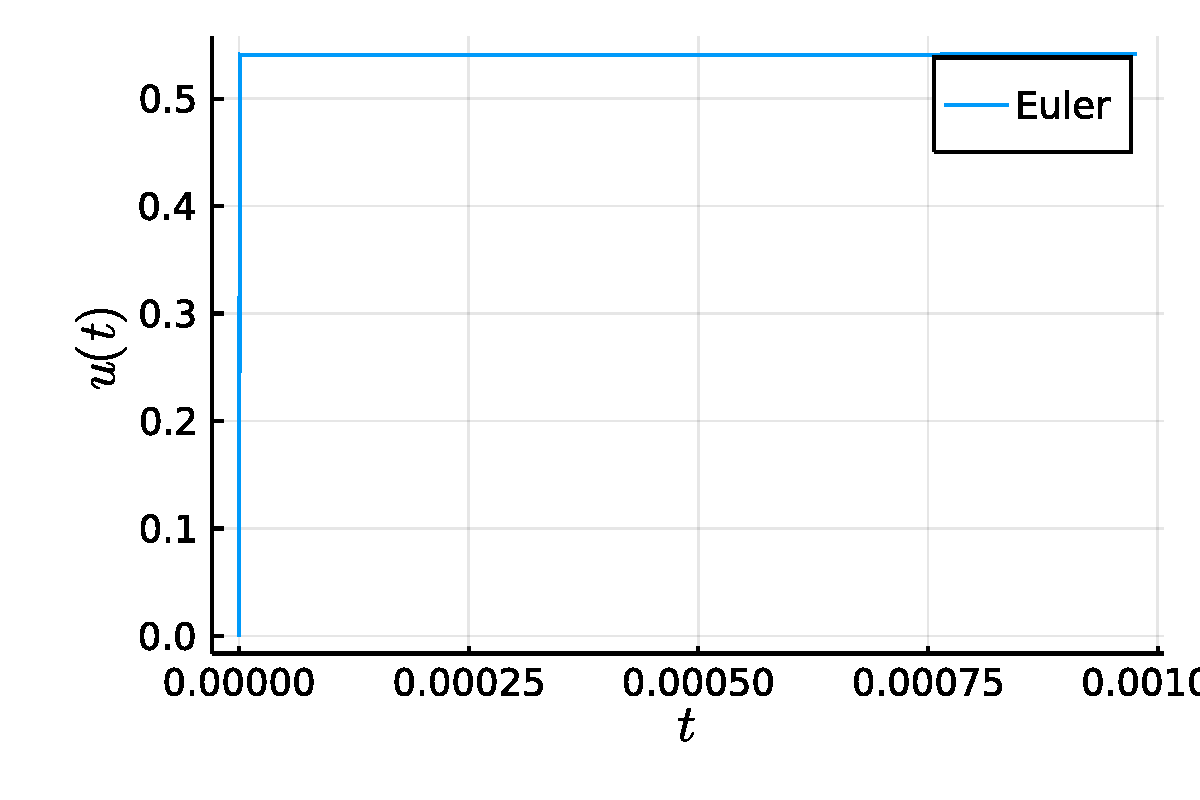
\includegraphics[width=\linewidth]{figures/ass_1_report_7_1.pdf}

\subsection{Part 2}
For backward Euler I explicitely defined the function and derivative for Newtons method.

\textbf{The solution for $T=10$ using backward Euler}


\begin{lstlisting}
(*@\HLJLcs{{\#}}@*) (*@\HLJLcs{Backward}@*) (*@\HLJLcs{Euler}@*)
(*@\HLJLk{function}@*) (*@\HLJLnf{BackwardEuler}@*)(*@\HLJLp{(}@*)(*@\HLJLn{N}@*)(*@\HLJLp{,}@*)(*@\HLJLn{T}@*)(*@\HLJLp{,}@*)(*@\HLJLn{t0}@*)(*@\HLJLp{,}@*)(*@\HLJLn{u0}@*)(*@\HLJLp{,}@*)(*@\HLJLn{\ensuremath{\lambda}}@*)(*@\HLJLp{)}@*)
    (*@\HLJLn{u}@*) (*@\HLJLoB{=}@*) (*@\HLJLnf{zeros}@*)(*@\HLJLp{(}@*)(*@\HLJLn{N}@*)(*@\HLJLoB{+}@*)(*@\HLJLni{1}@*)(*@\HLJLp{)}@*)
    (*@\HLJLn{u}@*)(*@\HLJLp{[}@*)(*@\HLJLni{1}@*)(*@\HLJLp{]}@*) (*@\HLJLoB{=}@*) (*@\HLJLn{u0}@*)
    (*@\HLJLn{h}@*) (*@\HLJLoB{=}@*) (*@\HLJLn{T}@*)(*@\HLJLoB{/}@*)(*@\HLJLn{N}@*)
    (*@\HLJLn{t}@*) (*@\HLJLoB{=}@*) (*@\HLJLn{t0}@*)
    (*@\HLJLn{x0}@*) (*@\HLJLoB{=}@*) (*@\HLJLnfB{2.0}@*)
    (*@\HLJLk{for}@*) (*@\HLJLn{i}@*) (*@\HLJLoB{=}@*) (*@\HLJLni{1}@*)(*@\HLJLoB{:}@*)(*@\HLJLn{N}@*)
        (*@\HLJLn{t}@*) (*@\HLJLoB{+=}@*) (*@\HLJLn{h}@*)
        (*@\HLJLnf{f}@*)(*@\HLJLp{(}@*)(*@\HLJLn{x}@*)(*@\HLJLp{,}@*) (*@\HLJLn{s}@*)(*@\HLJLp{)}@*) (*@\HLJLoB{=}@*) (*@\HLJLn{u}@*)(*@\HLJLp{[}@*)(*@\HLJLn{i}@*)(*@\HLJLp{]}@*) (*@\HLJLoB{+}@*) (*@\HLJLn{h}@*)(*@\HLJLoB{*}@*)(*@\HLJLp{(}@*)(*@\HLJLoB{-}@*)(*@\HLJLn{\ensuremath{\lambda}}@*)(*@\HLJLoB{*}@*)(*@\HLJLnf{sinh}@*)(*@\HLJLp{(}@*)(*@\HLJLn{x}@*)(*@\HLJLoB{-}@*)(*@\HLJLnf{cos}@*)(*@\HLJLp{(}@*)(*@\HLJLn{t}@*)(*@\HLJLoB{-}@*)(*@\HLJLni{1}@*)(*@\HLJLp{)))}@*)
        (*@\HLJLnf{df}@*)(*@\HLJLp{(}@*)(*@\HLJLn{x}@*)(*@\HLJLp{,}@*)(*@\HLJLn{s}@*)(*@\HLJLp{)}@*) (*@\HLJLoB{=}@*) (*@\HLJLoB{-}@*)(*@\HLJLn{\ensuremath{\lambda}}@*)(*@\HLJLoB{*}@*)(*@\HLJLn{h}@*)(*@\HLJLoB{*}@*)(*@\HLJLnf{cosh}@*)(*@\HLJLp{(}@*)(*@\HLJLn{x}@*)(*@\HLJLoB{-}@*)(*@\HLJLnf{cos}@*)(*@\HLJLp{(}@*)(*@\HLJLn{t}@*)(*@\HLJLoB{-}@*)(*@\HLJLni{1}@*)(*@\HLJLp{))}@*) (*@\HLJLoB{-}@*) (*@\HLJLni{1}@*)

        (*@\HLJLn{u}@*)(*@\HLJLp{[}@*)(*@\HLJLn{i}@*)(*@\HLJLoB{+}@*)(*@\HLJLni{1}@*)(*@\HLJLp{]}@*) (*@\HLJLoB{=}@*) (*@\HLJLnf{Newtons}@*)(*@\HLJLp{(}@*)(*@\HLJLn{f}@*)(*@\HLJLp{,}@*) (*@\HLJLn{df}@*)(*@\HLJLp{,}@*) (*@\HLJLn{x0}@*)(*@\HLJLp{,}@*) (*@\HLJLni{1}@*)(*@\HLJLp{)}@*)
    (*@\HLJLk{end}@*)

    (*@\HLJLk{return}@*) (*@\HLJLn{u}@*)
(*@\HLJLk{end}@*)

(*@\HLJLn{T}@*) (*@\HLJLoB{=}@*) (*@\HLJLnfB{10.0}@*)(*@\HLJLp{;}@*) (*@\HLJLn{t0}@*) (*@\HLJLoB{=}@*) (*@\HLJLnfB{0.0}@*)(*@\HLJLp{;}@*) (*@\HLJLn{u0}@*) (*@\HLJLoB{=}@*) (*@\HLJLni{0}@*)(*@\HLJLp{;}@*) (*@\HLJLn{\ensuremath{\lambda}}@*) (*@\HLJLoB{=}@*) (*@\HLJLnfB{10.0}@*)(*@\HLJLoB{{\textasciicircum}}@*)(*@\HLJLp{(}@*)(*@\HLJLnfB{6.0}@*)(*@\HLJLp{);}@*) (*@\HLJLn{h}@*) (*@\HLJLoB{=}@*) (*@\HLJLnfB{0.1}@*)(*@\HLJLp{;}@*)
(*@\HLJLn{N}@*) (*@\HLJLoB{=}@*) (*@\HLJLnf{Int}@*)(*@\HLJLp{(}@*)(*@\HLJLn{T}@*)(*@\HLJLoB{/}@*)(*@\HLJLn{h}@*)(*@\HLJLp{)}@*)

(*@\HLJLcs{{\#}}@*) (*@\HLJLcs{u}@*) (*@\HLJLcs{=}@*) (*@\HLJLcs{DiffyQ.BackwardEuler(N,T,t0,u0,\ensuremath{\lambda})}@*)
(*@\HLJLn{u}@*) (*@\HLJLoB{=}@*) (*@\HLJLnf{BackwardEuler}@*)(*@\HLJLp{(}@*)(*@\HLJLn{N}@*)(*@\HLJLp{,}@*)(*@\HLJLn{T}@*)(*@\HLJLp{,}@*)(*@\HLJLn{t0}@*)(*@\HLJLp{,}@*)(*@\HLJLn{u0}@*)(*@\HLJLp{,}@*)(*@\HLJLn{\ensuremath{\lambda}}@*)(*@\HLJLp{)}@*)
(*@\HLJLn{tList}@*) (*@\HLJLoB{=}@*) (*@\HLJLnf{collect}@*)(*@\HLJLp{(}@*)(*@\HLJLni{0}@*)(*@\HLJLoB{:}@*)(*@\HLJLn{N}@*)(*@\HLJLp{)}@*)(*@\HLJLoB{*}@*)(*@\HLJLp{(}@*)(*@\HLJLn{T}@*)(*@\HLJLoB{/}@*)(*@\HLJLn{N}@*)(*@\HLJLp{)}@*)
(*@\HLJLcs{{\#}}@*) (*@\HLJLcs{tList}@*) (*@\HLJLcs{=}@*) (*@\HLJLcs{t0:h:T+t0}@*)
(*@\HLJLnf{plot}@*)(*@\HLJLp{(}@*)(*@\HLJLn{tList}@*)(*@\HLJLp{,}@*) (*@\HLJLn{u}@*)(*@\HLJLp{,}@*) (*@\HLJLn{label}@*) (*@\HLJLoB{=}@*) (*@\HLJLs{"{}backward}@*) (*@\HLJLs{Euler"{}}@*)(*@\HLJLp{)}@*)
(*@\HLJLnf{xlabel!}@*)(*@\HLJLp{(}@*)(*@\HLJLso{L"{}t"{}}@*)(*@\HLJLp{,}@*) (*@\HLJLn{thickness{\_}scaling}@*) (*@\HLJLoB{=}@*) (*@\HLJLnfB{1.5}@*)(*@\HLJLp{)}@*)
(*@\HLJLnf{ylabel!}@*)(*@\HLJLp{(}@*)(*@\HLJLso{L"{}u(t)"{}}@*)(*@\HLJLp{)}@*)
\end{lstlisting}

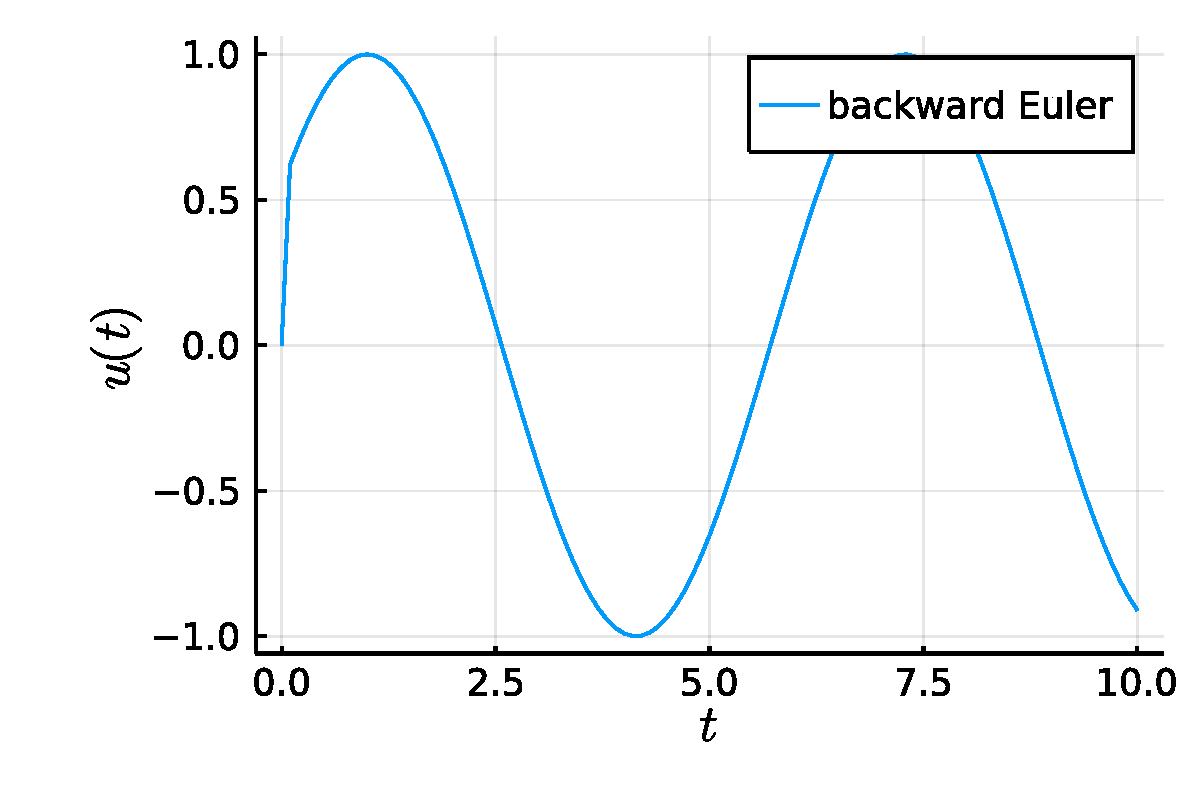
\includegraphics[width=\linewidth]{figures/ass_1_report_8_1.pdf}

\section{Problem 5}
Like backward Euler the Trapezoid method is also implicit, so I explicitely define the method here.

\subsection{Part 1}
\textbf{The solution for $T=10$ and $h=0.1$}


\begin{lstlisting}
(*@\HLJLcs{{\#}}@*) (*@\HLJLcs{The}@*) (*@\HLJLcs{differential}@*) (*@\HLJLcs{equation}@*) (*@\HLJLcs{to}@*) (*@\HLJLcs{be}@*) (*@\HLJLcs{solved}@*)
(*@\HLJLnf{func}@*)(*@\HLJLp{(}@*)(*@\HLJLn{u}@*)(*@\HLJLp{,}@*) (*@\HLJLn{t}@*)(*@\HLJLp{,}@*) (*@\HLJLn{\ensuremath{\lambda}}@*)(*@\HLJLp{)}@*) (*@\HLJLoB{=}@*) (*@\HLJLoB{-}@*)(*@\HLJLn{\ensuremath{\lambda}}@*)(*@\HLJLoB{*}@*)(*@\HLJLnf{sinh}@*)(*@\HLJLp{(}@*)(*@\HLJLn{u}@*)(*@\HLJLoB{-}@*)(*@\HLJLnf{cos}@*)(*@\HLJLp{(}@*)(*@\HLJLn{t}@*)(*@\HLJLoB{-}@*)(*@\HLJLni{1}@*)(*@\HLJLp{))}@*)

(*@\HLJLk{function}@*) (*@\HLJLnf{Trapezoid}@*)(*@\HLJLp{(}@*)(*@\HLJLn{N}@*)(*@\HLJLp{,}@*)(*@\HLJLn{T}@*)(*@\HLJLp{,}@*)(*@\HLJLn{t0}@*)(*@\HLJLp{,}@*) (*@\HLJLn{u0}@*)(*@\HLJLp{,}@*) (*@\HLJLn{\ensuremath{\lambda}}@*)(*@\HLJLp{)}@*)
    (*@\HLJLcs{{\#}}@*) (*@\HLJLcs{u}@*) (*@\HLJLcs{=}@*) (*@\HLJLcs{spzeros(N)}@*)
    (*@\HLJLn{u}@*) (*@\HLJLoB{=}@*) (*@\HLJLnf{zeros}@*)(*@\HLJLp{(}@*)(*@\HLJLn{N}@*)(*@\HLJLoB{+}@*)(*@\HLJLni{1}@*)(*@\HLJLp{)}@*)
    (*@\HLJLn{u}@*)(*@\HLJLp{[}@*)(*@\HLJLni{1}@*)(*@\HLJLp{]}@*) (*@\HLJLoB{=}@*) (*@\HLJLn{u0}@*)
    (*@\HLJLn{h}@*) (*@\HLJLoB{=}@*) (*@\HLJLn{T}@*)(*@\HLJLoB{/}@*)(*@\HLJLn{N}@*)
    (*@\HLJLn{t}@*) (*@\HLJLoB{=}@*) (*@\HLJLn{t0}@*)
    (*@\HLJLk{for}@*) (*@\HLJLn{i}@*) (*@\HLJLoB{=}@*) (*@\HLJLni{1}@*)(*@\HLJLoB{:}@*)(*@\HLJLn{N}@*)
        (*@\HLJLn{t}@*) (*@\HLJLoB{+=}@*) (*@\HLJLn{h}@*)
        (*@\HLJLcs{{\#}}@*) (*@\HLJLcs{Use}@*) (*@\HLJLcs{Newtons}@*) (*@\HLJLcs{Method}@*) (*@\HLJLcs{to}@*) (*@\HLJLcs{solve}@*) (*@\HLJLcs{nonlinear}@*) (*@\HLJLcs{eqn}@*) (*@\HLJLcs{for}@*) (*@\HLJLcs{u[n+1]}@*)
        (*@\HLJLnf{f}@*)(*@\HLJLp{(}@*)(*@\HLJLn{x}@*)(*@\HLJLp{,}@*)(*@\HLJLn{s}@*)(*@\HLJLp{)}@*) (*@\HLJLoB{=}@*) (*@\HLJLn{u}@*)(*@\HLJLp{[}@*)(*@\HLJLn{i}@*)(*@\HLJLp{]}@*) (*@\HLJLoB{+}@*) (*@\HLJLn{h}@*)(*@\HLJLoB{/}@*)(*@\HLJLni{2}@*) (*@\HLJLoB{*}@*) (*@\HLJLp{(}@*)(*@\HLJLnf{func}@*)(*@\HLJLp{(}@*)(*@\HLJLn{u}@*)(*@\HLJLp{[}@*)(*@\HLJLn{i}@*)(*@\HLJLp{],}@*)(*@\HLJLn{t}@*)(*@\HLJLoB{-}@*)(*@\HLJLn{h}@*)(*@\HLJLp{,}@*)(*@\HLJLn{\ensuremath{\lambda}}@*)(*@\HLJLp{)}@*) (*@\HLJLoB{-}@*) (*@\HLJLn{\ensuremath{\lambda}}@*)(*@\HLJLoB{*}@*)(*@\HLJLnf{sinh}@*)(*@\HLJLp{(}@*)(*@\HLJLn{x}@*)(*@\HLJLoB{-}@*)(*@\HLJLnf{cos}@*)(*@\HLJLp{(}@*)(*@\HLJLn{t}@*)(*@\HLJLoB{-}@*)(*@\HLJLni{1}@*)(*@\HLJLp{)))}@*) (*@\HLJLoB{-}@*) (*@\HLJLn{x}@*)
        (*@\HLJLnf{df}@*)(*@\HLJLp{(}@*)(*@\HLJLn{x}@*)(*@\HLJLp{,}@*)(*@\HLJLn{s}@*)(*@\HLJLp{)}@*) (*@\HLJLoB{=}@*) (*@\HLJLoB{-}@*)(*@\HLJLn{\ensuremath{\lambda}}@*)(*@\HLJLoB{*}@*)(*@\HLJLn{h}@*)(*@\HLJLoB{/}@*)(*@\HLJLni{2}@*)(*@\HLJLoB{*}@*)(*@\HLJLnf{cosh}@*)(*@\HLJLp{(}@*)(*@\HLJLn{x}@*)(*@\HLJLoB{-}@*)(*@\HLJLnf{cos}@*)(*@\HLJLp{(}@*)(*@\HLJLn{t}@*)(*@\HLJLoB{-}@*)(*@\HLJLni{1}@*)(*@\HLJLp{))}@*) (*@\HLJLoB{-}@*) (*@\HLJLni{1}@*)
        (*@\HLJLn{u}@*)(*@\HLJLp{[}@*)(*@\HLJLn{i}@*)(*@\HLJLoB{+}@*)(*@\HLJLni{1}@*)(*@\HLJLp{]}@*) (*@\HLJLoB{=}@*) (*@\HLJLnf{Newtons}@*)(*@\HLJLp{(}@*)(*@\HLJLn{f}@*)(*@\HLJLp{,}@*)(*@\HLJLn{df}@*)(*@\HLJLp{,}@*)(*@\HLJLnfB{2.0}@*)(*@\HLJLp{,}@*)(*@\HLJLnfB{1.0}@*)(*@\HLJLp{)}@*)
    (*@\HLJLk{end}@*)
    (*@\HLJLk{return}@*) (*@\HLJLn{u}@*)
(*@\HLJLk{end}@*)

(*@\HLJLn{T}@*) (*@\HLJLoB{=}@*) (*@\HLJLni{10}@*)(*@\HLJLp{;}@*) (*@\HLJLn{t0}@*) (*@\HLJLoB{=}@*) (*@\HLJLni{0}@*)(*@\HLJLp{;}@*) (*@\HLJLn{u0}@*) (*@\HLJLoB{=}@*) (*@\HLJLni{0}@*)(*@\HLJLp{;}@*) (*@\HLJLn{\ensuremath{\lambda}}@*) (*@\HLJLoB{=}@*) (*@\HLJLnfB{10.0}@*)(*@\HLJLoB{{\textasciicircum}}@*)(*@\HLJLp{(}@*)(*@\HLJLnfB{6.0}@*)(*@\HLJLp{);}@*)

(*@\HLJLn{h}@*) (*@\HLJLoB{=}@*) (*@\HLJLnfB{0.1}@*)
(*@\HLJLn{N}@*) (*@\HLJLoB{=}@*) (*@\HLJLnf{Int}@*)(*@\HLJLp{(}@*)(*@\HLJLn{T}@*)(*@\HLJLoB{/}@*)(*@\HLJLn{h}@*)(*@\HLJLp{)}@*)

(*@\HLJLn{u}@*) (*@\HLJLoB{=}@*) (*@\HLJLnf{Trapezoid}@*)(*@\HLJLp{(}@*)(*@\HLJLn{N}@*)(*@\HLJLp{,}@*)(*@\HLJLn{T}@*)(*@\HLJLp{,}@*)(*@\HLJLn{t0}@*)(*@\HLJLp{,}@*)(*@\HLJLn{u0}@*)(*@\HLJLp{,}@*)(*@\HLJLn{\ensuremath{\lambda}}@*)(*@\HLJLp{)}@*)
(*@\HLJLn{tList}@*) (*@\HLJLoB{=}@*) (*@\HLJLnf{collect}@*)(*@\HLJLp{(}@*)(*@\HLJLni{0}@*)(*@\HLJLoB{:}@*)(*@\HLJLn{N}@*)(*@\HLJLp{)}@*)(*@\HLJLoB{*}@*)(*@\HLJLp{(}@*)(*@\HLJLn{T}@*)(*@\HLJLoB{/}@*)(*@\HLJLn{N}@*)(*@\HLJLp{)}@*)
(*@\HLJLnf{plot}@*)(*@\HLJLp{(}@*)(*@\HLJLn{tList}@*)(*@\HLJLp{,}@*) (*@\HLJLn{u}@*)(*@\HLJLp{,}@*) (*@\HLJLn{label}@*) (*@\HLJLoB{=}@*) (*@\HLJLs{"{}Trapezoid"{}}@*)(*@\HLJLp{)}@*)
(*@\HLJLnf{xlabel!}@*)(*@\HLJLp{(}@*)(*@\HLJLso{L"{}t"{}}@*)(*@\HLJLp{,}@*) (*@\HLJLn{thickness{\_}scaling}@*) (*@\HLJLoB{=}@*) (*@\HLJLnfB{1.5}@*)(*@\HLJLp{)}@*)
(*@\HLJLnf{ylabel!}@*)(*@\HLJLp{(}@*)(*@\HLJLn{L}@*)(*@\HLJLs{"{}u(t)"{}}@*)(*@\HLJLp{)}@*)
\end{lstlisting}

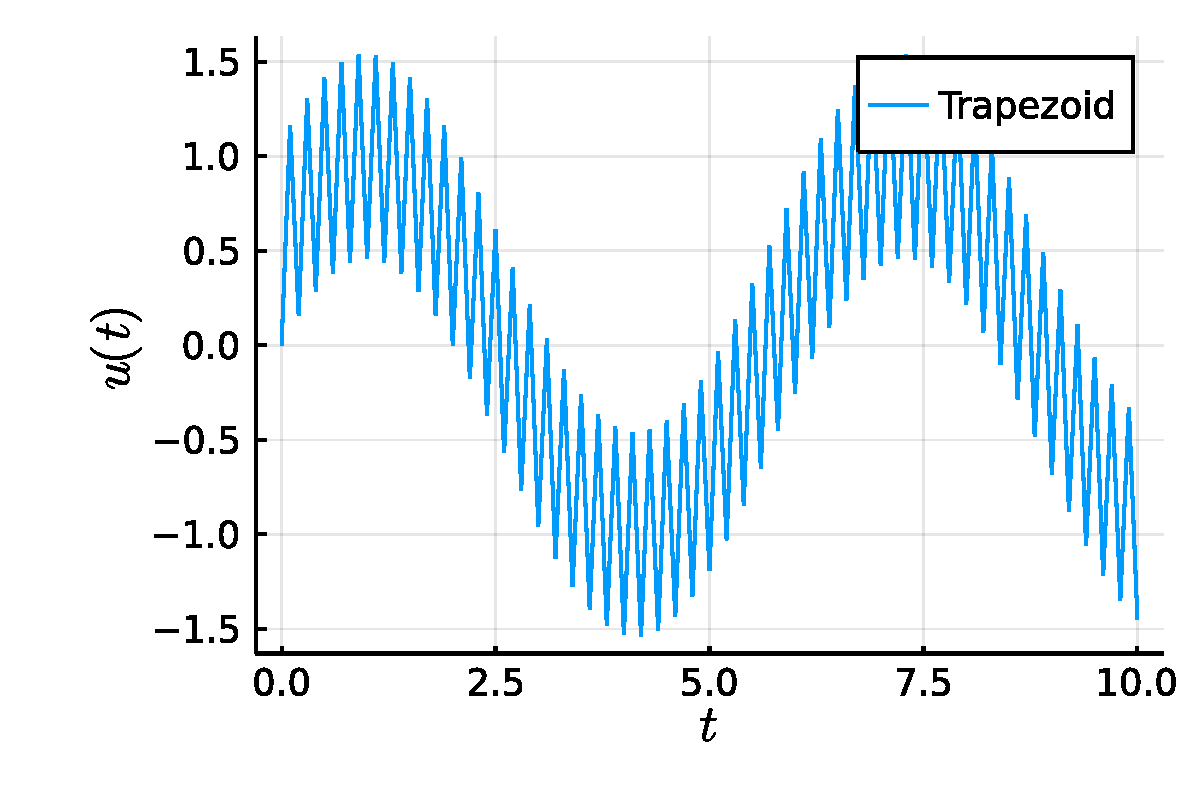
\includegraphics[width=\linewidth]{figures/ass_1_report_9_1.pdf}

This method seems to oscillate around the solution.

\subsection{Part 2}
\textbf{Plotting smaller and smaller stepsizes, we can see how the solution behaves}


\begin{lstlisting}
(*@\HLJLk{for}@*) (*@\HLJLn{i}@*) (*@\HLJLoB{=}@*) (*@\HLJLni{7}@*)(*@\HLJLoB{:}@*)(*@\HLJLni{2}@*)(*@\HLJLoB{:}@*)(*@\HLJLni{12}@*)
    (*@\HLJLkd{local}@*) (*@\HLJLn{h}@*) (*@\HLJLoB{=}@*) (*@\HLJLnfB{2.0}@*)(*@\HLJLoB{{\textasciicircum}}@*)(*@\HLJLp{(}@*)(*@\HLJLoB{-}@*)(*@\HLJLn{i}@*)(*@\HLJLp{)}@*)
    (*@\HLJLkd{local}@*) (*@\HLJLn{N}@*) (*@\HLJLoB{=}@*) (*@\HLJLnf{Int}@*)(*@\HLJLp{(}@*)(*@\HLJLn{T}@*)(*@\HLJLoB{/}@*)(*@\HLJLn{h}@*)(*@\HLJLp{)}@*)
    (*@\HLJLkd{local}@*) (*@\HLJLn{u}@*) (*@\HLJLoB{=}@*) (*@\HLJLnf{Trapezoid}@*)(*@\HLJLp{(}@*)(*@\HLJLn{N}@*)(*@\HLJLp{,}@*)(*@\HLJLn{T}@*)(*@\HLJLp{,}@*)(*@\HLJLn{t0}@*)(*@\HLJLp{,}@*)(*@\HLJLn{u0}@*)(*@\HLJLp{,}@*)(*@\HLJLn{\ensuremath{\lambda}}@*)(*@\HLJLp{)}@*)
    (*@\HLJLkd{local}@*) (*@\HLJLn{tList}@*) (*@\HLJLoB{=}@*) (*@\HLJLnf{collect}@*)(*@\HLJLp{(}@*)(*@\HLJLni{0}@*)(*@\HLJLoB{:}@*)(*@\HLJLn{N}@*)(*@\HLJLp{)}@*)(*@\HLJLoB{*}@*)(*@\HLJLp{(}@*)(*@\HLJLn{T}@*)(*@\HLJLoB{/}@*)(*@\HLJLn{N}@*)(*@\HLJLp{)}@*)
    (*@\HLJLnf{display}@*)(*@\HLJLp{(}@*)(*@\HLJLnf{plot}@*)(*@\HLJLp{(}@*)(*@\HLJLn{tList}@*)(*@\HLJLp{,}@*) (*@\HLJLn{u}@*)(*@\HLJLp{,}@*) (*@\HLJLn{label}@*) (*@\HLJLoB{=}@*) (*@\HLJLs{"{}Trapezoid"{}}@*)(*@\HLJLp{,}@*) (*@\HLJLn{xlabel}@*) (*@\HLJLoB{=}@*) (*@\HLJLso{L"{}t"{}}@*)(*@\HLJLp{,}@*) (*@\HLJLn{thickness{\_}scaling}@*) (*@\HLJLoB{=}@*) (*@\HLJLnfB{1.5}@*)(*@\HLJLp{,}@*) (*@\HLJLn{ylabel}@*)(*@\HLJLoB{=}@*) (*@\HLJLso{L"{}u(t)"{}}@*)(*@\HLJLp{))}@*)
(*@\HLJLk{end}@*)
\end{lstlisting}

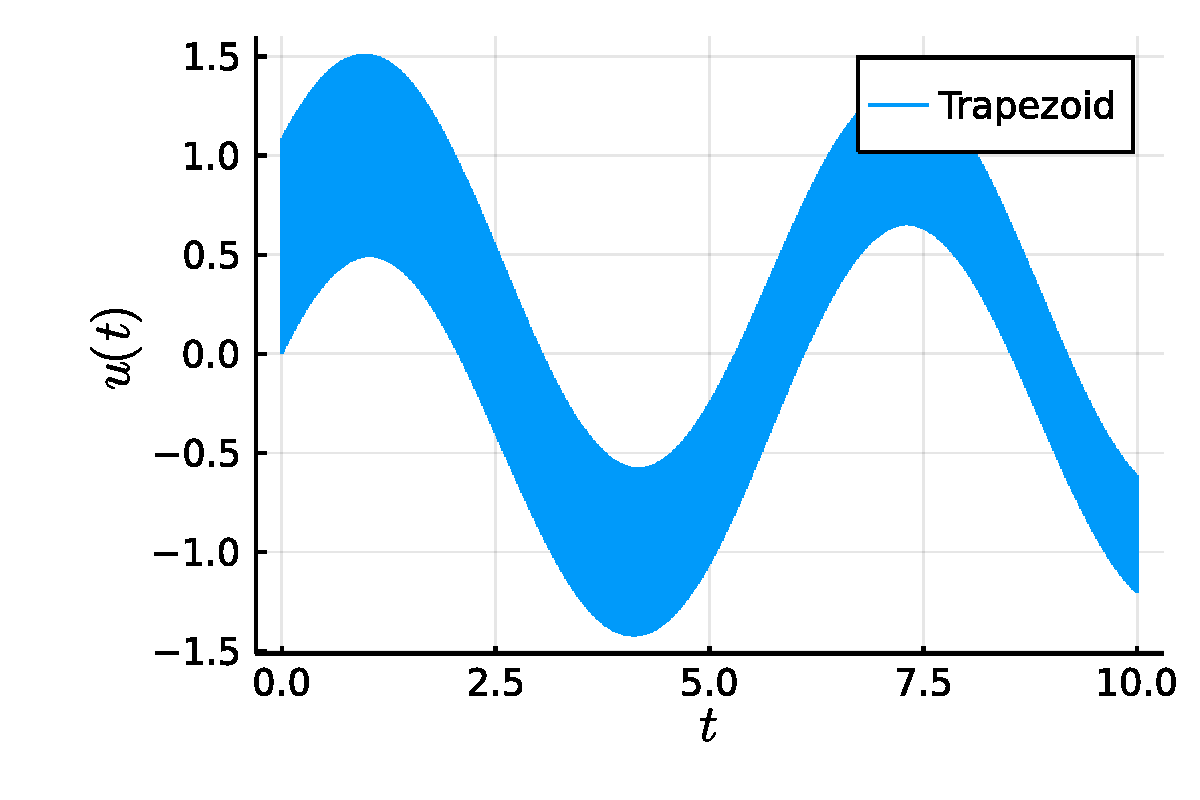
\includegraphics[width=\linewidth]{figures/ass_1_report_10_1.pdf}
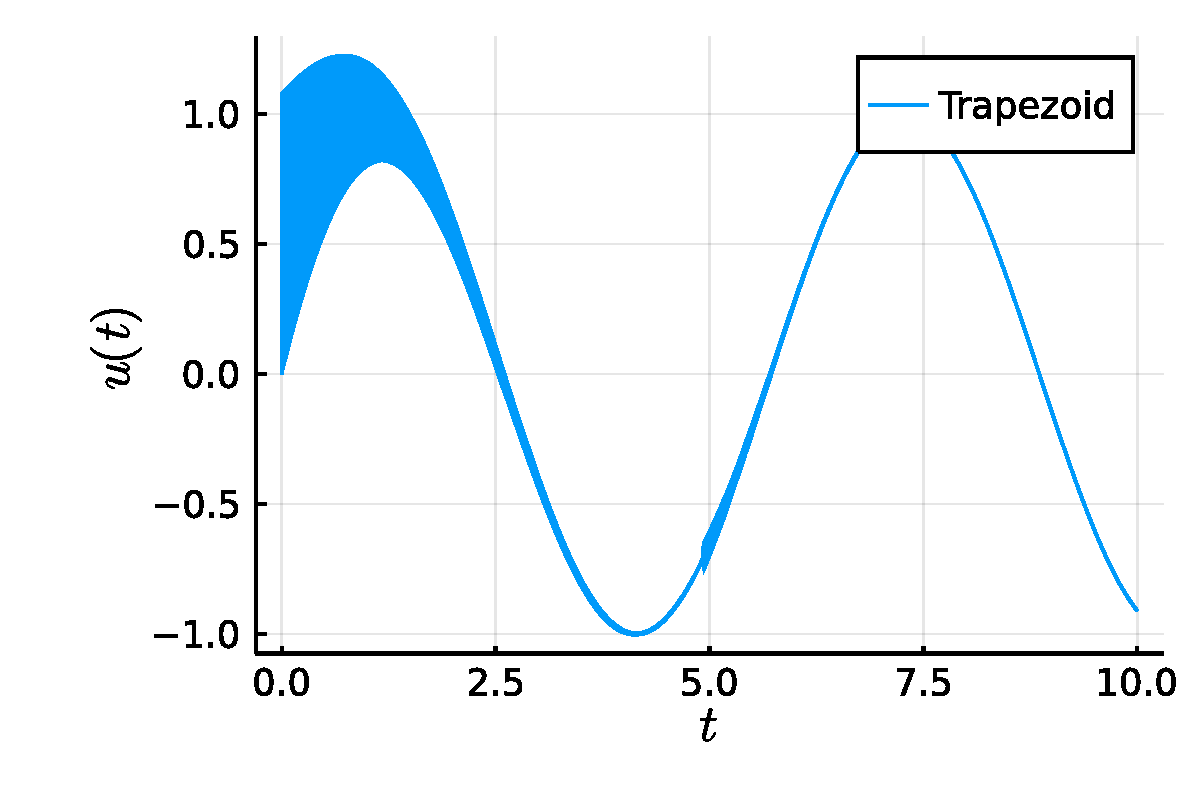
\includegraphics[width=\linewidth]{figures/ass_1_report_10_2.pdf}
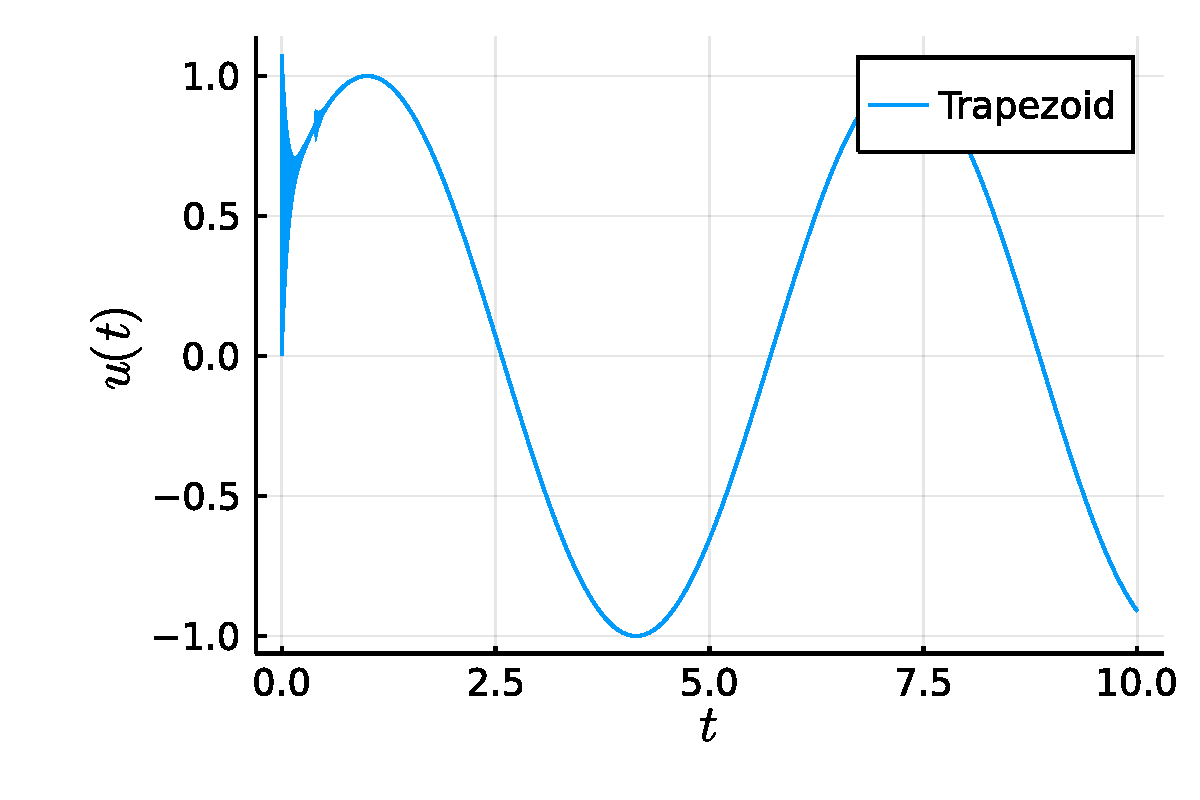
\includegraphics[width=\linewidth]{figures/ass_1_report_10_3.pdf}

The oscillations dissipate and the method converges to the solution.

\section{Problem 6}
\subsection{Part 1}
\textbf{Plotting Euler's method and 2-step Midpoint rule for $T = 2$ and $h=0.2$}


\begin{lstlisting}
(*@\HLJLnf{func}@*)(*@\HLJLp{(}@*)(*@\HLJLn{u}@*)(*@\HLJLp{,}@*)(*@\HLJLn{t}@*)(*@\HLJLp{,}@*) (*@\HLJLn{\ensuremath{\lambda}}@*)(*@\HLJLp{)}@*) (*@\HLJLoB{=}@*) (*@\HLJLoB{-}@*)(*@\HLJLn{u}@*)

(*@\HLJLn{T}@*) (*@\HLJLoB{=}@*) (*@\HLJLni{2}@*)(*@\HLJLp{;}@*) (*@\HLJLn{h}@*) (*@\HLJLoB{=}@*) (*@\HLJLnfB{0.2}@*)(*@\HLJLp{;}@*) (*@\HLJLn{t0}@*) (*@\HLJLoB{=}@*) (*@\HLJLni{0}@*)(*@\HLJLp{;}@*)
(*@\HLJLn{N}@*) (*@\HLJLoB{=}@*) (*@\HLJLnf{Int}@*)(*@\HLJLp{(}@*)(*@\HLJLn{T}@*)(*@\HLJLoB{/}@*)(*@\HLJLn{h}@*)(*@\HLJLp{)}@*)
(*@\HLJLnf{uexact}@*)(*@\HLJLp{(}@*)(*@\HLJLn{t}@*)(*@\HLJLp{)}@*) (*@\HLJLoB{=}@*) (*@\HLJLnf{exp}@*)(*@\HLJLp{(}@*)(*@\HLJLoB{-}@*)(*@\HLJLn{t}@*)(*@\HLJLp{)}@*)
(*@\HLJLn{u0}@*) (*@\HLJLoB{=}@*) (*@\HLJLni{1}@*)
(*@\HLJLn{u1}@*) (*@\HLJLoB{=}@*) (*@\HLJLnf{uexact}@*)(*@\HLJLp{(}@*)(*@\HLJLn{h}@*)(*@\HLJLp{)}@*)

(*@\HLJLn{umid}@*) (*@\HLJLoB{=}@*) (*@\HLJLnf{Midpoint2Step}@*)(*@\HLJLp{(}@*)(*@\HLJLn{func}@*)(*@\HLJLp{,}@*) (*@\HLJLn{N}@*)(*@\HLJLp{,}@*) (*@\HLJLn{T}@*)(*@\HLJLp{,}@*) (*@\HLJLn{t0}@*)(*@\HLJLp{,}@*) (*@\HLJLn{u0}@*)(*@\HLJLp{,}@*) (*@\HLJLn{u1}@*)(*@\HLJLp{)}@*)
(*@\HLJLn{ueul}@*) (*@\HLJLoB{=}@*) (*@\HLJLnf{Euler}@*)(*@\HLJLp{(}@*)(*@\HLJLn{func}@*)(*@\HLJLp{,}@*) (*@\HLJLn{N}@*)(*@\HLJLp{,}@*) (*@\HLJLn{T}@*)(*@\HLJLp{,}@*) (*@\HLJLn{t0}@*)(*@\HLJLp{,}@*) (*@\HLJLn{u0}@*)(*@\HLJLp{)}@*)

(*@\HLJLn{tList}@*) (*@\HLJLoB{=}@*) (*@\HLJLnf{collect}@*)(*@\HLJLp{(}@*)(*@\HLJLni{0}@*)(*@\HLJLoB{:}@*)(*@\HLJLn{N}@*)(*@\HLJLp{)}@*)(*@\HLJLoB{*}@*)(*@\HLJLp{(}@*)(*@\HLJLn{T}@*)(*@\HLJLoB{/}@*)(*@\HLJLn{N}@*)(*@\HLJLp{)}@*)
(*@\HLJLnf{plot}@*)(*@\HLJLp{(}@*)(*@\HLJLn{tList}@*)(*@\HLJLp{,}@*)(*@\HLJLn{umid}@*)(*@\HLJLp{,}@*) (*@\HLJLn{label}@*) (*@\HLJLoB{=}@*) (*@\HLJLs{"{}Midpoint"{}}@*)(*@\HLJLp{)}@*)
(*@\HLJLnf{plot!}@*)(*@\HLJLp{(}@*)(*@\HLJLn{tList}@*)(*@\HLJLp{,}@*)(*@\HLJLn{ueul}@*)(*@\HLJLp{,}@*) (*@\HLJLn{label}@*) (*@\HLJLoB{=}@*) (*@\HLJLs{"{}Euler"{}}@*)(*@\HLJLp{)}@*)
(*@\HLJLnf{plot!}@*)(*@\HLJLp{(}@*)(*@\HLJLn{tList}@*)(*@\HLJLp{,}@*)(*@\HLJLn{uexact}@*)(*@\HLJLoB{.}@*)(*@\HLJLp{(}@*)(*@\HLJLn{tList}@*)(*@\HLJLp{),}@*) (*@\HLJLn{label}@*) (*@\HLJLoB{=}@*) (*@\HLJLs{"{}Exact"{}}@*)(*@\HLJLp{,}@*) (*@\HLJLn{marker}@*) (*@\HLJLoB{=}@*) (*@\HLJLp{(}@*)(*@\HLJLsc{:dot}@*)(*@\HLJLp{,}@*)(*@\HLJLnfB{1.5}@*)(*@\HLJLp{),}@*) (*@\HLJLn{add{\_}marker}@*)(*@\HLJLoB{=}@*)(*@\HLJLkc{true}@*)(*@\HLJLp{)}@*)
\end{lstlisting}

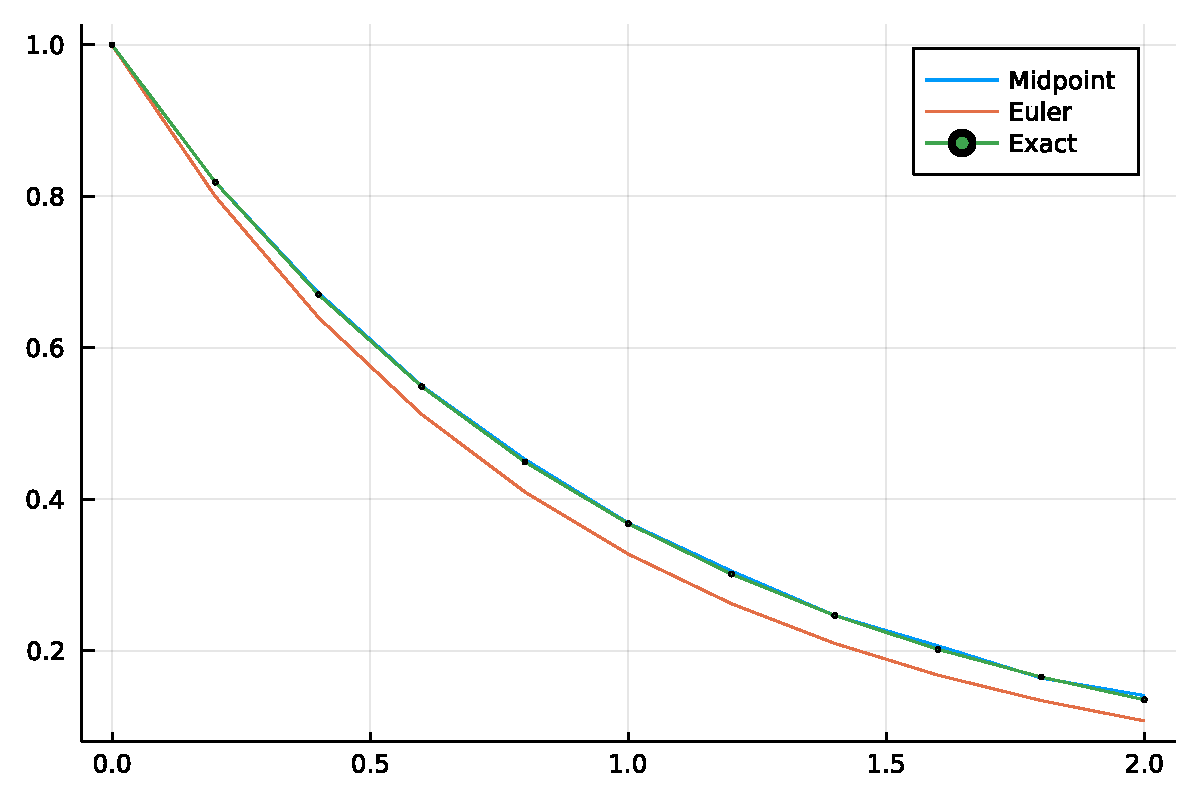
\includegraphics[width=\linewidth]{figures/ass_1_report_11_1.pdf}

\textbf{The midpoint method is more accurate in this time period.}

\subsection{Part 2}
\textbf{Ploting now over a longer time period $T = 20$}


\begin{lstlisting}
(*@\HLJLn{T}@*) (*@\HLJLoB{=}@*) (*@\HLJLnfB{20.0}@*)
(*@\HLJLn{N}@*) (*@\HLJLoB{=}@*) (*@\HLJLnf{Int}@*)(*@\HLJLp{(}@*)(*@\HLJLn{T}@*)(*@\HLJLoB{/}@*)(*@\HLJLn{h}@*)(*@\HLJLp{)}@*)

(*@\HLJLn{umid}@*) (*@\HLJLoB{=}@*) (*@\HLJLnf{Midpoint2Step}@*)(*@\HLJLp{(}@*)(*@\HLJLn{func}@*)(*@\HLJLp{,}@*) (*@\HLJLn{N}@*)(*@\HLJLp{,}@*) (*@\HLJLn{T}@*)(*@\HLJLp{,}@*) (*@\HLJLn{t0}@*)(*@\HLJLp{,}@*) (*@\HLJLn{u0}@*)(*@\HLJLp{,}@*) (*@\HLJLn{u1}@*)(*@\HLJLp{)}@*)
(*@\HLJLn{ueul}@*) (*@\HLJLoB{=}@*) (*@\HLJLnf{Euler}@*)(*@\HLJLp{(}@*)(*@\HLJLn{func}@*)(*@\HLJLp{,}@*) (*@\HLJLn{N}@*)(*@\HLJLp{,}@*) (*@\HLJLn{T}@*)(*@\HLJLp{,}@*) (*@\HLJLn{t0}@*)(*@\HLJLp{,}@*) (*@\HLJLn{u0}@*)(*@\HLJLp{)}@*)

(*@\HLJLn{tList}@*) (*@\HLJLoB{=}@*) (*@\HLJLnf{collect}@*)(*@\HLJLp{(}@*)(*@\HLJLni{0}@*)(*@\HLJLoB{:}@*)(*@\HLJLn{N}@*)(*@\HLJLp{)}@*)(*@\HLJLoB{*}@*)(*@\HLJLp{(}@*)(*@\HLJLn{T}@*)(*@\HLJLoB{/}@*)(*@\HLJLn{N}@*)(*@\HLJLp{)}@*)
(*@\HLJLnf{plot}@*)(*@\HLJLp{(}@*)(*@\HLJLn{tList}@*)(*@\HLJLp{,}@*)(*@\HLJLn{umid}@*)(*@\HLJLp{,}@*) (*@\HLJLn{label}@*) (*@\HLJLoB{=}@*) (*@\HLJLs{"{}Midpoint"{}}@*)(*@\HLJLp{)}@*)
(*@\HLJLnf{plot!}@*)(*@\HLJLp{(}@*)(*@\HLJLn{tList}@*)(*@\HLJLp{,}@*)(*@\HLJLn{ueul}@*)(*@\HLJLp{,}@*) (*@\HLJLn{label}@*) (*@\HLJLoB{=}@*) (*@\HLJLs{"{}Euler"{}}@*)(*@\HLJLp{)}@*)
\end{lstlisting}

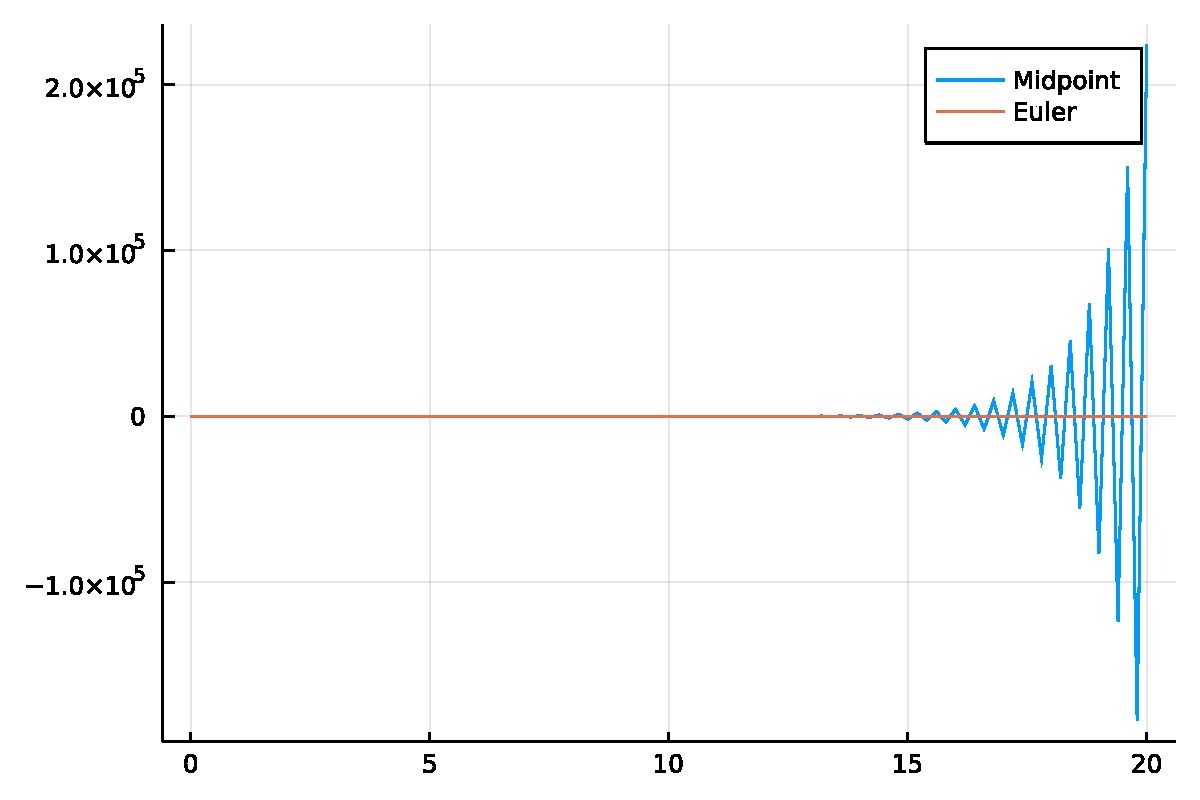
\includegraphics[width=\linewidth]{figures/ass_1_report_12_1.pdf}

\textbf{The midpoint method is not well behaved.}

\subsection{Part 3}
\textbf{Reducing now the timestep for the same time period $T=20$}


\begin{lstlisting}
(*@\HLJLk{for}@*) (*@\HLJLn{i}@*) (*@\HLJLoB{=}@*) (*@\HLJLni{5}@*)(*@\HLJLoB{:}@*)(*@\HLJLni{7}@*)
    (*@\HLJLkd{local}@*) (*@\HLJLn{h}@*) (*@\HLJLoB{=}@*) (*@\HLJLnfB{0.2}@*)(*@\HLJLoB{/}@*)(*@\HLJLp{(}@*)(*@\HLJLni{2}@*)(*@\HLJLoB{{\textasciicircum}}@*)(*@\HLJLn{i}@*)(*@\HLJLp{)}@*)
    (*@\HLJLkd{local}@*) (*@\HLJLn{N}@*) (*@\HLJLoB{=}@*) (*@\HLJLnf{Int}@*)(*@\HLJLp{(}@*)(*@\HLJLn{T}@*)(*@\HLJLoB{/}@*)(*@\HLJLn{h}@*)(*@\HLJLp{)}@*)
    (*@\HLJLkd{local}@*) (*@\HLJLn{umid}@*) (*@\HLJLoB{=}@*) (*@\HLJLnf{Midpoint2Step}@*)(*@\HLJLp{(}@*)(*@\HLJLn{func}@*)(*@\HLJLp{,}@*) (*@\HLJLn{N}@*)(*@\HLJLp{,}@*) (*@\HLJLn{T}@*)(*@\HLJLp{,}@*) (*@\HLJLn{t0}@*)(*@\HLJLp{,}@*) (*@\HLJLn{u0}@*)(*@\HLJLp{,}@*) (*@\HLJLn{u1}@*)(*@\HLJLp{)}@*)
    (*@\HLJLkd{local}@*) (*@\HLJLn{ueul}@*) (*@\HLJLoB{=}@*) (*@\HLJLnf{Euler}@*)(*@\HLJLp{(}@*)(*@\HLJLn{func}@*)(*@\HLJLp{,}@*) (*@\HLJLn{N}@*)(*@\HLJLp{,}@*) (*@\HLJLn{T}@*)(*@\HLJLp{,}@*) (*@\HLJLn{t0}@*)(*@\HLJLp{,}@*) (*@\HLJLn{u0}@*)(*@\HLJLp{)}@*)

    (*@\HLJLkd{local}@*) (*@\HLJLn{tList}@*) (*@\HLJLoB{=}@*) (*@\HLJLnf{collect}@*)(*@\HLJLp{(}@*)(*@\HLJLni{0}@*)(*@\HLJLoB{:}@*)(*@\HLJLn{N}@*)(*@\HLJLp{)}@*)(*@\HLJLoB{*}@*)(*@\HLJLp{(}@*)(*@\HLJLn{T}@*)(*@\HLJLoB{/}@*)(*@\HLJLn{N}@*)(*@\HLJLp{)}@*)
    (*@\HLJLkd{local}@*) (*@\HLJLn{p1}@*) (*@\HLJLoB{=}@*) (*@\HLJLnf{plot}@*)(*@\HLJLp{(}@*)(*@\HLJLn{tList}@*)(*@\HLJLp{,}@*)(*@\HLJLn{umid}@*)(*@\HLJLp{,}@*) (*@\HLJLn{label}@*) (*@\HLJLoB{=}@*) (*@\HLJLs{"{}Midpoint"{}}@*)(*@\HLJLp{)}@*)
    (*@\HLJLkd{local}@*) (*@\HLJLn{p2}@*) (*@\HLJLoB{=}@*) (*@\HLJLnf{plot!}@*)(*@\HLJLp{(}@*)(*@\HLJLn{tList}@*)(*@\HLJLp{,}@*)(*@\HLJLn{ueul}@*)(*@\HLJLp{,}@*) (*@\HLJLn{label}@*) (*@\HLJLoB{=}@*) (*@\HLJLs{"{}Euler"{}}@*)(*@\HLJLp{)}@*)
    (*@\HLJLnf{display}@*)(*@\HLJLp{(}@*)(*@\HLJLn{p2}@*)(*@\HLJLp{)}@*)
(*@\HLJLk{end}@*)
\end{lstlisting}

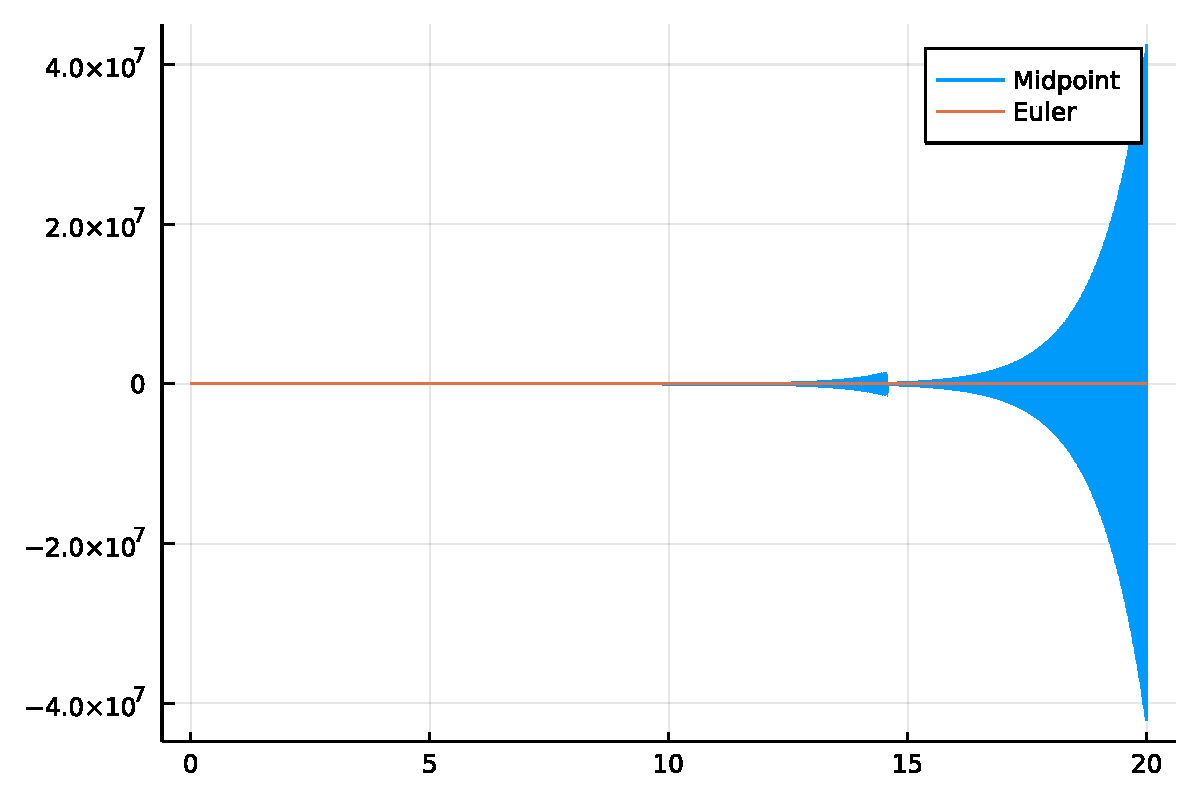
\includegraphics[width=\linewidth]{figures/ass_1_report_13_1.pdf}
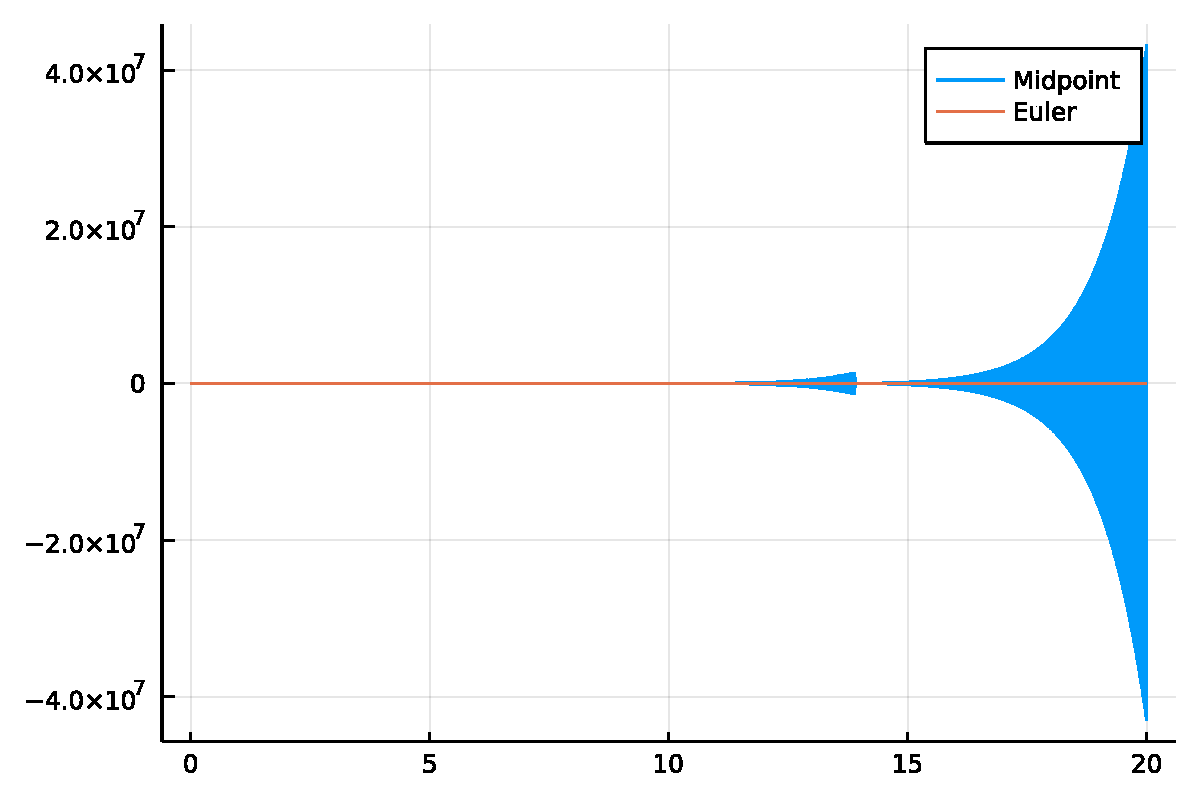
\includegraphics[width=\linewidth]{figures/ass_1_report_13_2.pdf}
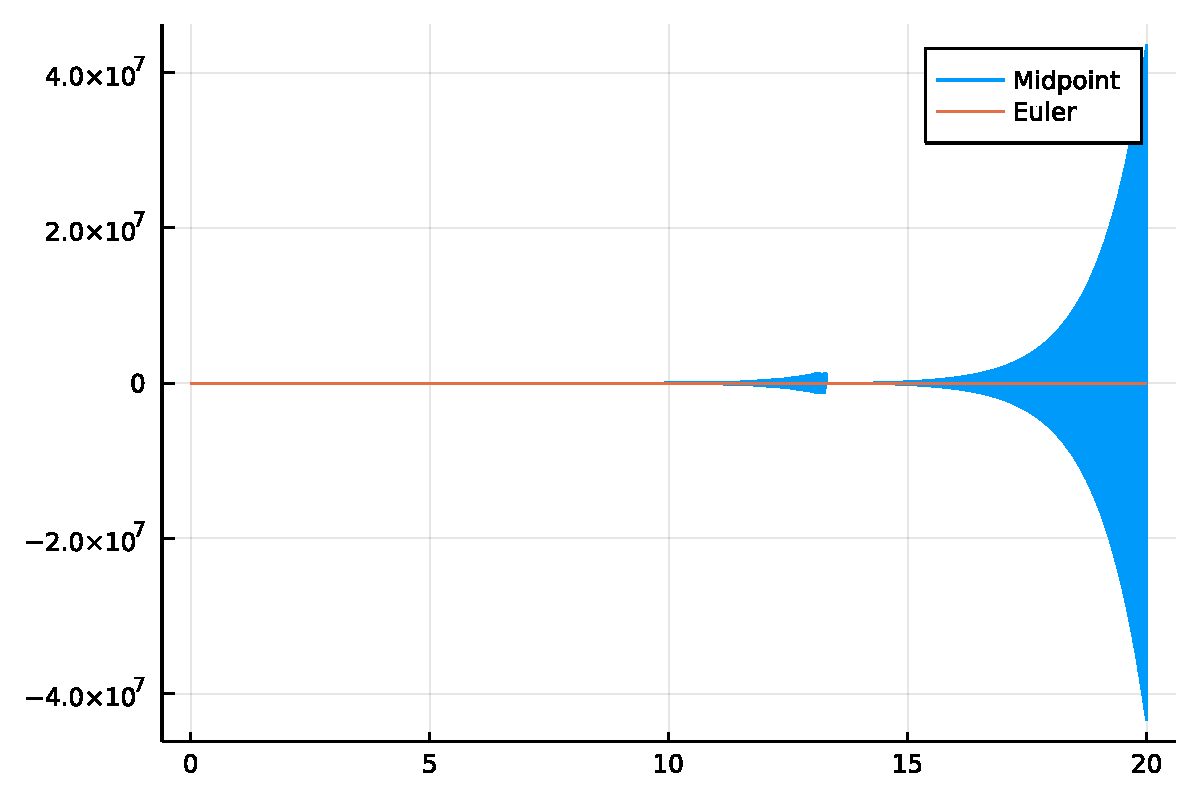
\includegraphics[width=\linewidth]{figures/ass_1_report_13_3.pdf}

\textbf{The midpoint method does not improve.}



\end{document}
